% ============================================================
%  ALP at FCC-ee Z-pole: projected constraints
%  Author: Iñaki Pardo
%  Draft — P6 Project Period 2025/2026
% ============================================================
\documentclass[12pt,a4paper]{article}

\usepackage[margin=2.5cm]{geometry}
\usepackage{amsmath,amssymb,amsfonts}
\usepackage{graphicx}
\usepackage{hyperref}
\usepackage{xcolor}
\usepackage{booktabs}
\usepackage{siunitx}
\usepackage{caption}
\usepackage{subcaption}
\usepackage{float}
\usepackage{tikz}
\usetikzlibrary{decorations.pathmorphing}
\usepackage[numbers,sort&compress]{natbib}
\usepackage{lineno}
\usepackage{setspace}

\onehalfspacing
\linenumbers

\hypersetup{colorlinks=true,linkcolor=blue,citecolor=blue,urlcolor=blue}

% ============================================================
\begin{document}

\title{\textbf{Searching for Axion-Like Particles at FCC-ee:\\
    Projected Sensitivity in the Invisible and Prompt-Resolved Channels\\
    at the Z Pole}}

\author{Iñaki Pardo\\
    \small Maastricht Science Programme, Maastricht University\\
    \small \texttt{inaxpardo0204@gmail.com}}

\date{June 2026 — Project Period Draft}
\maketitle

% ============================================================
\begin{abstract}
We present projected sensitivity estimates for the production of axion-like
particles (ALPs) at the proposed Future Circular Collider operating at the
Z~pole ($\sqrt{s} = 91.2\,\text{GeV}$, $\mathcal{L} = 150\,\text{ab}^{-1}$) via the associated
production process $e^+e^- \to \gamma\,a$.
Two detector signatures are analyzed: the \emph{invisible} channel, in which
the ALP escapes the detector ($\ell_a > L_\mathrm{max}$), and the
\emph{prompt-resolved} channel, in which the ALP decays to two separated
photons inside the tracker ($\ell_a < L_\mathrm{min}$,
$\Delta\theta > \Delta\theta_\mathrm{res}$).
Signal events are generated with \textsc{MadGraph5\_{aMC@NLO}}, processed
through \textsc{Pythia\,8} for ALP decay and lifetime, and passed through
a \textsc{Delphes} fast simulation of the IDEA detector concept.
SM backgrounds for both channels are simulated, binned, and normalized to the
full target luminosity.
Projected 90\% CL exclusion contours are derived using a binned
Asimov $\Delta\chi^2$ method, with analytic production and lifetime formulas corrected
by detector-level signal scans.
For the invisible channel, the analysis reaches
$g_{a\gamma\gamma} \approx 5.5\times10^{-7}\,\text{GeV}^{-1}$ over the ALP mass range
$0.01\text{--}0.92\,\text{GeV}$.
The prompt-resolved channel extends sensitivity to
$g_{a\gamma\gamma} \sim 10^{-5}\text{--}3\times10^{-4}\,\text{GeV}^{-1}$ for
$m_{a} \in [0.61, 80]\,\text{GeV}$.
Both projected contours surpass current collider bounds by one to two orders
of magnitude in coupling at comparable masses.
The analysis machinery is validated against the published Belle~II
ALP exclusion boundary, reproducing it to within
$|\log_{10}(g_\mathrm{closure}/g_\mathrm{published})| \leq 7.6\times10^{-3}$.
Additional validation gates check the MadGraph cross section, the ALP width and
Pythia lifetime convention, the Delphes output, and the reconstructed ALP
invariant-mass or recoil-energy observable at every detector-level signal point.
\end{abstract}

% ============================================================
\section{Introduction}
\label{sec:intro}

The Peccei--Quinn (PQ) mechanism, proposed to explain the absence of
strong CP violation~\cite{Peccei1977,Weinberg1978,Wilczek1978}, predicts the
existence of a pseudo-Nambu--Goldstone boson, the axion.
The simplest requirement for the PQ mechanism to resolve the strong CP problem
constrains the axion mass and its couplings to a narrow band in the coupling--mass
plane---the so-called QCD axion line.
However, extensions of this framework that decouple the mass from the
coupling give rise to \emph{axion-like particles} (ALPs): pseudo-scalars that
couple to Standard Model (SM) particles with arbitrary mass--coupling
combinations~\cite{Jaeckel2010,Brivio2017,Dolan2017}.

The ALP--photon coupling,
\begin{equation}
    \mathcal{L} \supset -\frac{1}{4}g_{a\gamma\gamma}\,a\,F_{\mu\nu}\tilde{F}^{\mu\nu},
    \label{eq:lagrangian}
\end{equation}
is particularly well-motivated.
It arises generically from the anomalous coupling of any axion-like field to
the electromagnetic field strength $F_{\mu\nu}$, and is bounded across many
orders of magnitude in mass by astrophysical, cosmological, and laboratory
experiments~\cite{AxionLimits}.
In the mass range $10\,\text{MeV}$--$80\,\text{GeV}$ relevant to collider searches,
the most stringent direct constraints come from $e^+e^-$ collider experiments
(LEP, Belle~II, BaBar, BESIII) and beam-dump experiments, and leave significant
regions of parameter space unexplored at couplings
$g_{a\gamma\gamma} \lesssim 10^{-4}\,\text{GeV}^{-1}$.

\begin{figure}[H]
    \centering
    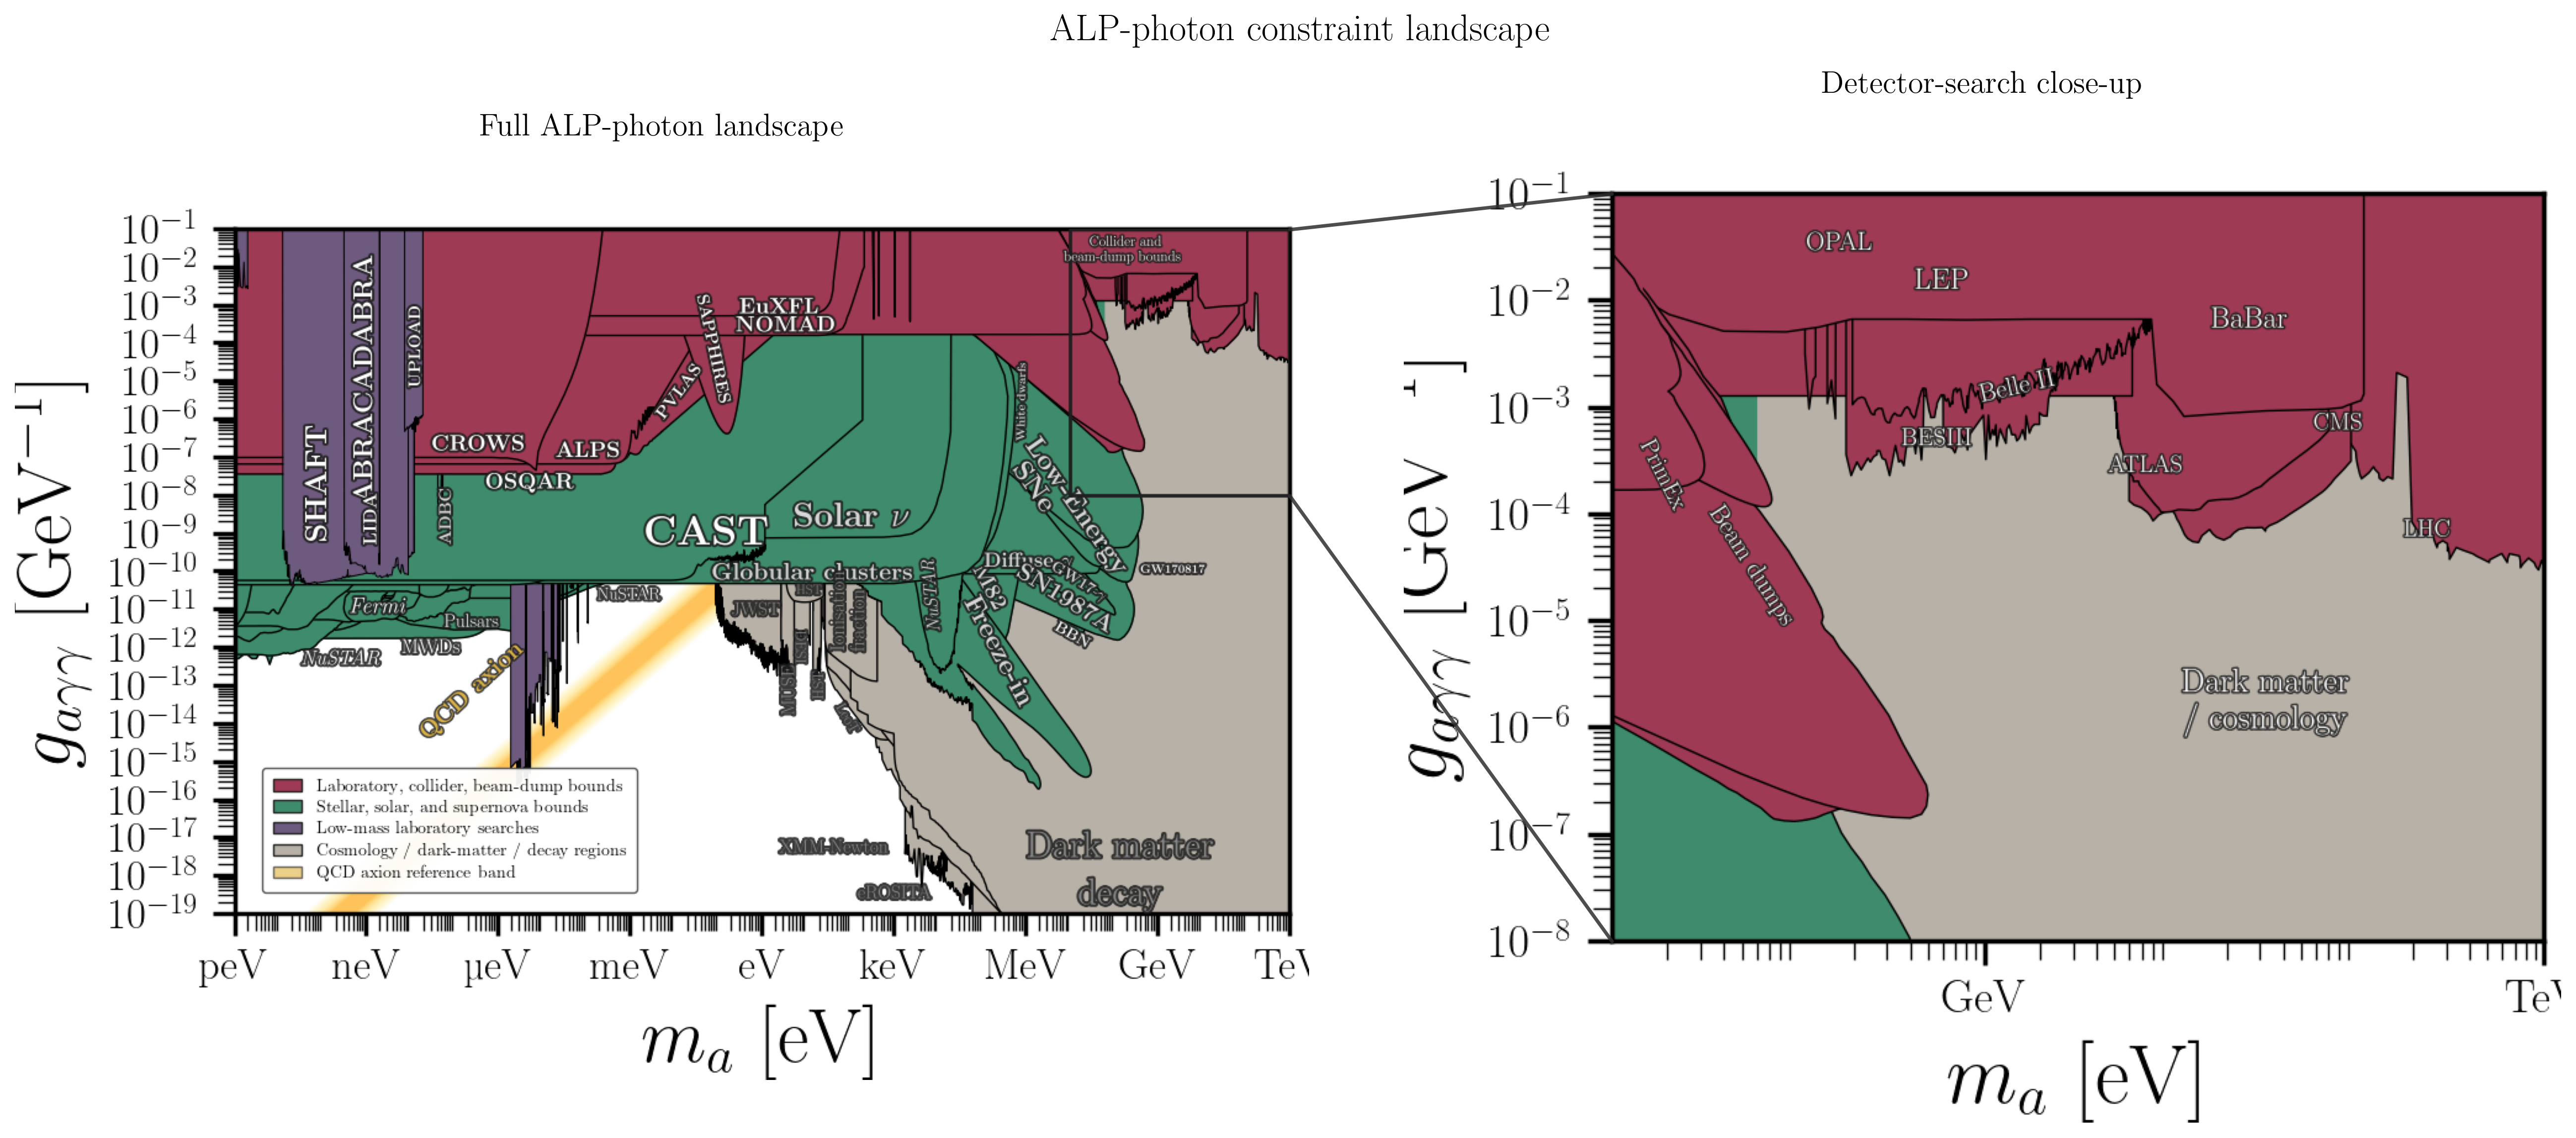
\includegraphics[width=\textwidth]{figures/axionlimits_alp_landscape_intro.png}
    \caption{Current ALP-photon constraint landscape used as context for this
    project, produced from the pinned AxionLimits repository. The left panel
    shows the broad landscape, while the right panel zooms into the
    collider-relevant mass range. Solid colored regions show existing
    laboratory, astrophysical, cosmological, and dark-matter-motivated
    constraints or reference regions. The FCC-ee projections are deliberately
    omitted here and are introduced later as the project result.}
    \label{fig:intro_landscape}
\end{figure}

The Future Circular Collider (FCC-ee) is a proposed $e^+e^-$ machine
that would operate at several center-of-mass energies from the Z pole
($\sqrt{s} \approx 91.2\,\text{GeV}$) up to the $t\bar{t}$ threshold~\cite{FCCee_CDR,FCC_Physics}.
At the Z pole, the baseline luminosity target of $150\,\text{ab}^{-1}$---corresponding
to approximately $5\times10^{12}$ Z bosons---provides an extraordinarily
clean and prolific environment for precision measurements and rare-process
searches.
For photophilic ALPs, the associated production cross section
$\sigma(e^+e^-\to\gamma\,a) \propto g_{a\gamma\gamma}^2(1-m_{a}^2/s)^3$ grows quadratically with the
coupling and benefits enormously from the high luminosity, making FCC-ee a
uniquely powerful probe.
The Z-pole run is chosen as the baseline deliverable for three practical and
physics reasons. First, it is the FCC-ee stage with the largest expected
integrated luminosity, so it gives the strongest statistics-driven reach for
the single-coupling process studied here. Second, the fixed center-of-mass
energy gives a simple mono-energetic recoil photon,
$E_\gamma=(s-m_{a}^2)/(2\sqrt{s})$, making the invisible and prompt-resolved
analyses especially transparent. Third, the Z-pole overlaps the mass range
where existing collider constraints from Belle~II, BaBar, BESIII, LEP, and the
LHC leave open regions that can be tested in a clean $e^+e^-$ environment.
Other FCC-ee stages are scientifically interesting, but each stage has a
different luminosity, background composition, recoil-energy range, and
detector acceptance optimization. They are therefore treated as extensions
rather than part of the controlled final deliverable.

This paper presents projected ALP sensitivity estimates at the FCC-ee
Z~pole, focusing on the two experimentally cleanest signatures: the
invisible channel (ALP escapes) and the prompt-resolved channel (ALP decays
to two separated photons).
The analysis uses a complete simulation chain from matrix-element
generation to fast detector response, validated against published experimental
results.

A central goal of the project is not only to draw an ALP sensitivity curve,
but to build a reusable ALP simulation and analysis pipeline.
This matters because an ALP search is not determined by the production formula
alone. The same point in the $(m_{a},g_{a\gamma\gamma})$ plane can look like missing energy,
three photons, two merged photon clusters, or a displaced decay depending on
the ALP lifetime and boost. The detector response then decides how many of
those ideal events are actually reconstructed, while Standard Model processes
decide how difficult the signal is to distinguish from ordinary events.
A pipeline that connects theory, event generation, detector simulation,
background modeling, and limit setting is therefore needed if the final
projection is to mean more than an idealized rate estimate. It also makes the
analysis extensible: the same structure can later be reused for other FCC-ee
energies, different detector assumptions, displaced or merged channels, or
additional ALP operators.

\paragraph{Paper structure.}
Section~\ref{sec:theory} reviews the relevant ALP physics.
Section~\ref{sec:simulation} describes the simulation and detector modeling.
Section~\ref{sec:analysis} presents the signal classification, background
estimation, and limit-setting method.
Section~\ref{sec:results} reports the projected exclusion contours.
Section~\ref{sec:discussion} discusses the physics reach, limitations, and outlook.

% ============================================================
\section{Theory}
\label{sec:theory}

\subsection{Analytic model for photophilic ALPs}

This analysis assumes a single effective operator,
Eq.~\eqref{eq:lagrangian}, with all direct ALP couplings to fermions, gluons,
$W$ bosons, and $Z$ bosons set to zero at tree level. The only model
parameters scanned are therefore the ALP mass $m_{a}$ and the photon coupling
$g_{a\gamma\gamma}$. To calculate any process we need to compute the amplitude of the
interaction. This is derived from the Lagrangian of the interaction
\eqref{eq:lagrangian}. In this benchmark the total width is taken to be
\begin{equation}
    \Gamma_\mathrm{tot} \simeq \Gamma(a\to\gamma\gamma),
    \label{eq:width_assumption}
\end{equation}
because $a\to\gamma\gamma$ is the only open tree-level decay channel in the
implemented model. Loop-induced fermion modes are neglected consistently with
the photophilic benchmark and with the UFO parameter choice used in the
simulation.

\subsection{Associated-production kinematics and amplitude}

In the center-of-mass frame, the total four-momentum of the collision is
$P^\mu=p_{e^-}^\mu+p_{e^+}^\mu=(\sqrt{s},0,0,0)$, where $\sqrt{s}$ is the
center-of-mass energy of the collision, and $p_{e^-}$ and $p_{e^+}$ are the
incoming electron and positron four-momenta. Momentum conservation tells us
that this is equal to the total four-momentum of the outgoing ALP and photon,
$P^\mu=p_a^\mu+k^\mu$, where $p_a$ is the outgoing ALP four-momentum and $k$
is the outgoing recoil-photon four-momentum. We then have $P^\mu-k^\mu=p_a^\mu$,
so squaring it gives
\begin{align}
    (P^\mu-k^\mu)(P_\mu-k_\mu)&=p_a^\mu p_{a\mu}
    \nonumber\\
    P^2-2P\cdot k+k^2&=p_a^{2}
    \nonumber\\
    s-2P\cdot k&=m_{a}^{2}
    \nonumber\\
    s-2(\sqrt{s}, \mathbf{0})\cdot (E_\gamma,\mathbf{k})&=m_{a}^{2}
    \nonumber\\
    s-2\sqrt{s} E_\gamma&=m_{a}^{2}.
    \label{eq:recoil_energy_derivation}
\end{align}
Here $k^2=0$ for the recoil photon, since photons are massless, and
$p_a^2=m_{a}^2$ for the ALP. So in the center-of-mass frame we can express the
recoil photon energy as
\begin{equation}
    E_{\gamma,\mathrm{recoil}}=\frac{s-m_{a}^2}{2\sqrt{s}}.
    \label{eq:Egamma}
\end{equation}
It follows that the ALP energy and the three-momentum magnitude are
\begin{equation}
    E_a
    =
    \sqrt{s}-E_\gamma
    =
    \frac{s+m_{a}^2}{2\sqrt{s}},
    \qquad
    |\mathbf{p}_a|
    =
    |\mathbf{k}|
    =
    \frac{s-m_{a}^2}{2\sqrt{s}}.
    \label{eq:two_body_kinematics}
\end{equation}
$E_{\gamma,\mathrm{recoil}}$ is therefore one of the main signals we use,
since we can reconstruct the invariant mass of the ALP when we detect the
recoil photon. At fixed $\sqrt{s}$ and $m_{a}$, a two-body final state has no
freedom to choose a different recoil-photon energy before detector smearing or
initial-state radiation. The ALP is boosted with respect to its rest frame, and
we can get the ALP boost from these kinematic variables as
\begin{equation}
    \gamma_a=\frac{E_a}{m_{a}},
    \qquad
    \beta_a\gamma_a=\frac{|\mathbf{p}_a|}{m_{a}}.
    \label{eq:boost}
\end{equation}

The cross section is the quantity that tells us how often the process of an
ALP being created via associated production in an $e^+e^-$ collision occurs
for a given beam luminosity, $N=\sigma\mathcal{L}$. We can calculate
$\sigma(e^+e^-\to a\gamma)$ by using Fermi's golden rule in relativistic
phase-space form:
\begin{equation}
    d\sigma
    =
    \frac{S}{4\sqrt{(p_1\cdot p_2)^2-m_1^2m_2^2}}
    \overline{|\mathcal{M}|^2}
    (2\pi)^4
    \delta^{(4)}
    \!\left(p_1+p_2-\sum_f p_f\right)
    \prod_f
    \frac{d^3\mathbf{p}_f}{(2\pi)^3\,2E_f}.
    \label{eq:scattering-fermi}
\end{equation}
Here $p_1$ and $p_2$ are the incoming electron and positron momenta, and $m_1$
and $m_2$ are their masses. The factor with the square root is the incoming
flux. The delta function enforces conservation of the total four-momentum, and
the factor $S$ is a symmetry factor that avoids double counting identical
particles in the final state. For $e^+e^-\to\gamma a$ the photon and ALP are
different particles, so $S=1$. The final product is the Lorentz-invariant
phase space available to the outgoing particles.

To compute any process, we first need its amplitude, which contains all of the
dynamical information. We obtain it by evaluating the relevant Feynman diagram.
The first vertex of the interaction is the basic QED current: the incoming
electron and positron annihilate into an off-shell photon,
$e^+e^-\to\gamma^\ast(q)$, where $q=p_{e^-}+p_{e^+}$ and $q^2=s$. This virtual
photon then produces the recoil photon and the ALP through the ALP--photon
interaction. The full associated-production process is therefore
\begin{equation}
    e^+ e^- \to \gamma\,a.
    \label{eq:production}
\end{equation}
From the coupling between the ALP and photons in Eq.~\eqref{eq:lagrangian}, we
can derive the ALP--photon vertex
\begin{equation}
    V^{\mu\nu}(k_1,k_2)
    =
    -ig_{a\gamma\gamma}\epsilon^{\mu\nu\alpha\beta}k_{1,\alpha}k_{2,\beta},
    \label{eq:vertex}
\end{equation}
where $\epsilon^{\mu\nu\alpha\beta}$ is the four-dimensional Levi-Civita
symbol. It is a completely antisymmetric object which encodes the CP-odd
nature of the ALP--photon interaction. Both photon four-momenta,
$k_1^\alpha$ and $k_2^\beta$, are taken incoming to the vertex. However, in
production, one of these photon legs is the virtual $\gamma^\ast$, so we
designate its four-momentum as $q$; and the other is the recoil photon
$\gamma_\mathrm{recoil}$, which is outgoing from the ALP vertex, so the
all-incoming momentum assigned to that leg is $-k$. The ALP--photon vertex is
then
\begin{equation}
    V^{\nu\rho}(q,-k)
    =
    -ig_{a\gamma\gamma}\epsilon^{\nu\rho\alpha\beta}q_\alpha(-k)_\beta
    =
    ig_{a\gamma\gamma}\epsilon^{\nu\rho\alpha\beta}q_\alpha k_\beta.
    \label{eq:production-vertex}
\end{equation}
This is why the vertex appears with a plus sign in the production amplitude.

The amplitude for $e^+e^-\to a\gamma$ is therefore obtained by multiplying all
the pieces of associated production: the ordinary QED current, the
virtual-photon propagator, the ALP--photon vertex, and the polarization vector
of the outgoing photon,
\begin{align}
    \mathcal{M}
    &=
    i
    \underbrace{\bar{v}(p_{e^+})(-ie\gamma^{\mu})u(p_{e^-})}
        _{\substack{e^+e^-\gamma^\ast\\ \mathrm{current}}}
    \underbrace{\left(\frac{-ig_{\mu \nu}}{s}\right)}
        _{\substack{\gamma^\ast\\ \mathrm{propagator}}}
    \underbrace{\left(ig_{a\gamma \gamma}\epsilon^{\nu \rho\alpha \beta}q_{\alpha}k_{\beta}\right)}
        _{\substack{\gamma^\ast\gamma a\\ \mathrm{vertex}}}
    \underbrace{\varepsilon ^{*}_{\rho}(k)}
        _{\substack{\mathrm{outgoing}\ \gamma\\ \mathrm{polarization}}}
    \nonumber\\
    &=
    \frac{eg_{a\gamma\gamma}}{s}
    \left[
      \bar v(p_{e^+})\gamma^\mu u(p_{e^-})
    \right]
    \epsilon_{\mu\nu\alpha\beta}
    q^\alpha k^\beta
    \varepsilon^{*\nu}(k).
    \label{eq:prod_amp}
\end{align}
Here we contracted the Lorentz indices with the metric and the overall phase
has been dropped, since only $|\mathcal{M}|^2$ enters the cross section. The
electric charge $e$ comes from the ordinary QED vertex where the
electron--positron pair annihilates into a virtual photon. The spinors
$u(p_{e^-})$ and $\bar v(p_{e^+})$ describe the incoming electron and positron,
and $\gamma^\mu$ is a Dirac matrix. The factor $1/s$ is the propagator of the
intermediate virtual photon after contracting with the photon-current indices.
The factor
$g_{a\gamma\gamma}\epsilon_{\mu\nu\alpha\beta}q^\alpha k^\beta$ is the
ALP--photon vertex from Eq.~\eqref{eq:production-vertex}. Finally,
$\varepsilon^{*\nu}(k)$ is the polarization vector of the observed outgoing
photon, since we have to specify the physical polarization state of the recoil
photon. Because the detector does not measure photon polarization, when
calculating the cross section we sum over the allowed photon polarizations.

We now want to square the amplitude. A useful way to do this is to separate
the electron current from the ALP--photon tensor, so we define
\begin{equation}
    J^\mu=\bar v(p_{e^+})\gamma^\mu u(p_{e^-}),
    \qquad
    A_{\mu\nu}=\epsilon_{\mu\nu\alpha\beta}q^\alpha k^\beta .
\end{equation}
The amplitude then looks like
\begin{equation}
    \mathcal{M}
    =
    \frac{eg_{a\gamma\gamma}}{s}J^\mu A_{\mu\nu}\varepsilon^{*\nu}(k).
\end{equation}
For a fixed incoming electron spin, incoming positron spin, and outgoing
photon polarization, the squared amplitude is
\begin{equation}
    |\mathcal{M}|^2
    =
    \frac{e^2g_{a\gamma\gamma}^2}{s^2}
    J^\mu J^{\mu' *}
    A_{\mu\nu}A_{\mu'\nu'}
    \varepsilon^{*\nu}(k)\varepsilon^{\nu'}(k).
    \label{eq:prod_m2_fixed}
\end{equation}
In the FCC-ee collision, the beams are unpolarized, so we do not know which
initial spin state was present. We therefore average over the two electron
spin states and the two positron spin states, giving a factor $1/4$. The
detector also does not measure the polarization of the final photon, so we sum
over the two physical final photon polarizations:
\begin{align}
    \overline{|\mathcal{M}|^2}
    &=
    \frac{e^2g_{a\gamma\gamma}^2}{s^2}
    \left[
      \frac{1}{4}
      \sum_{s_-,s_+}
      J^\mu J^{\mu' *}
    \right]
    A_{\mu\nu}A_{\mu'\nu'}
    \left[
      \sum_\lambda
      \varepsilon^{*\nu}_{(\lambda)}(k)
      \varepsilon^{\nu'}_{(\lambda)}(k)
    \right].
    \label{eq:prod_m2_sums}
\end{align}
The object in the first bracket is the spin-averaged electron tensor, which
can be evaluated with the standard Dirac trace identities:
\begin{align}
    L^{\mu\mu'}
    &\equiv
    \frac{1}{4}
    \sum_{s_-,s_+}
    J^\mu J^{\mu' *}
    \nonumber\\
    &=
    \frac{1}{4}
    \mathrm{Tr}\!\left[
      (p_{e^+}\!\cdot\gamma)\gamma^\mu
      (p_{e^-}\!\cdot\gamma)\gamma^{\mu'}
    \right] \nonumber\\
    &=
    p_{e^+}^{\mu}p_{e^-}^{\mu'}
    +
    p_{e^+}^{\mu'}p_{e^-}^{\mu}
    -
    g^{\mu\mu'}(p_{e^+}\cdot p_{e^-}).
    \label{eq:leptonic_tensor}
\end{align}
This is the standard QED trace result in the limit where $m_e^2\ll s$. The
photon polarization sum in the second square bracket can be replaced by
$-g^{\nu\nu'}$, and gauge-dependent terms vanish because the amplitude is gauge
invariant. With these two results Eq.~\eqref{eq:prod_m2_sums} becomes
\begin{equation}
    \overline{|\mathcal{M}|^2}
    =
    \frac{e^2g_{a\gamma\gamma}^2}{s^2}
    L^{\mu\mu'}
    A_{\mu\nu}A_{\mu'\nu'}
    \left(-g^{\nu\nu'}\right).
    \label{eq:prod_m2_tensor}
\end{equation}
In the center-of-mass frame we can choose the incoming electron to define the
$z$-axis:
\begin{align}
    p_{e^-}^\mu
    &=
    \frac{\sqrt{s}}{2}(1,0,0,1),
    &
    p_{e^+}^\mu
    &=
    \frac{\sqrt{s}}{2}(1,0,0,-1),
    \nonumber\\
    q^\mu
    &=
    (\sqrt{s},0,0,0),
    &
    k^\mu
    &=
    E_\gamma(1,\sin\theta_\mathrm{CM},0,\cos\theta_\mathrm{CM}).
    \label{eq:cm_momenta}
\end{align}
Substituting these momenta into Eqs.~\eqref{eq:prod_m2_tensor} and
\eqref{eq:leptonic_tensor} gives
\begin{equation}
    \overline{|\mathcal{M}|^2}
    =
    e^2g_{a\gamma\gamma}^2 E_\gamma^2
    \left(1+\cos^2\theta_\mathrm{CM}\right).
    \label{eq:prod_m2_egamma}
\end{equation}
And finally, using $E_\gamma=(\sqrt{s}/2)(1-m_{a}^2/s)$ gives us
\begin{equation}
    \overline{|\mathcal{M}|^2}
    =
    \frac{e^2g_{a\gamma\gamma}^2s}{4}
    \left(1+\cos^2\theta_\mathrm{CM}\right)
    \left(1-\frac{m_{a}^2}{s}\right)^2,
    \label{eq:prod_m2}
\end{equation}
where $\theta_\mathrm{CM}$ is the recoil-photon polar angle relative to the
incoming electron direction. The factor $(1+\cos^2\theta_\mathrm{CM})$ gives
the angular shape, while $(1-m_{a}^2/s)^2$ shows the momentum dependence of the
pseudoscalar vertex. Plugging this squared amplitude into Fermi's golden rule
(Eq.~\eqref{eq:scattering-fermi}), we now reduce the two-body phase space and
obtain the differential cross section.

For associated production the final-state momenta are
\begin{equation}
    p_3=k
    \qquad\text{and}\qquad
    p_4=p_a,
\end{equation}
with $k^2=0$ for the photon and $p_a^2=m_{a}^2$ for the ALP. The electron mass
is negligible compared with the collider energy, so in the center-of-mass
frame $m_1=m_2\simeq0$ and
\begin{equation}
    4\sqrt{(p_1\cdot p_2)^2-m_1^2m_2^2}
    =
    4|\mathbf{p}_i|\sqrt{s}.
    \label{eq:flux_factor_cm}
\end{equation}
The two-body phase-space part of Eq.~\eqref{eq:scattering-fermi} is
\begin{equation}
    d\Phi_2
    =
    (2\pi)^4\delta^{(4)}(p_1+p_2-k-p_a)
    \frac{d^3\mathbf{k}}{(2\pi)^3\,2E_\gamma}
    \frac{d^3\mathbf{p}_a}{(2\pi)^3\,2E_a}.
    \label{eq:two_body_phase_space}
\end{equation}
In the center-of-mass frame the spatial delta function sets the two final
momenta to be back-to-back, $\mathbf{p}_a=-\mathbf{k}$. The remaining energy
delta function fixes the magnitude of the final momentum to the value already
found from two-body kinematics,
\begin{equation}
    |\mathbf{p}_f|
    =
    |\mathbf{k}|
    =
    \frac{s-m_{a}^2}{2\sqrt{s}}.
\end{equation}
After using the delta functions, the two-body phase space becomes
\begin{equation}
    d\Phi_2
    =
    \frac{1}{16\pi^2}
    \frac{|\mathbf{p}_f|}{\sqrt{s}}
    d\Omega,
    \label{eq:two_body_phase_space_reduced}
\end{equation}
where $d\Omega$ is the solid-angle element of the outgoing photon. Plugging
Eqs.~\eqref{eq:flux_factor_cm} and
\eqref{eq:two_body_phase_space_reduced} into
Eq.~\eqref{eq:scattering-fermi} gives the standard two-body formula for
unpolarized $2\to2$ scattering:
\begin{equation}
    \frac{d\sigma}{d\Omega}
    =
    \frac{1}{64\pi^2s}
    \frac{|\mathbf{p}_f|}{|\mathbf{p}_i|}
    \overline{|\mathcal{M}|^2},
    \label{eq:two_body_xsec}
\end{equation}
Here $|\mathbf{p}_i|=\sqrt{s}/2$ is the magnitude of the incoming electron or
positron three-momentum, and $|\mathbf{p}_f|$ is the magnitude of either
final-state momentum. The ratio $|\mathbf{p}_f|/|\mathbf{p}_i|$ is the
two-body phase-space suppression: if $m_{a}$ approaches $\sqrt{s}$, there is
little momentum left for the final state. Since
\begin{equation}
    \frac{|\mathbf{p}_f|}{|\mathbf{p}_i|}
    =
    1-\frac{m_{a}^2}{s},
\end{equation}
substituting Eq.~\eqref{eq:prod_m2} into Eq.~\eqref{eq:two_body_xsec} gives
\begin{align}
    \frac{d\sigma}{d\Omega}
    &=
    \frac{1}{64\pi^2s}
    \left(1-\frac{m_{a}^2}{s}\right)
    \frac{e^2g_{a\gamma\gamma}^2s}{4}
    \left(1+\cos^2\theta_\mathrm{CM}\right)
    \left(1-\frac{m_{a}^2}{s}\right)^2
    \nonumber\\
    &=
    \frac{e^2g_{a\gamma\gamma}^2}{256\pi^2}
    \left(1+\cos^2\theta_\mathrm{CM}\right)
    \left(1-\frac{m_{a}^2}{s}\right)^3.
    \label{eq:dsigma_domega_step}
\end{align}
There is no dependence on the azimuthal angle $\phi$ because the initial state
is rotationally symmetric around the beam axis. Therefore
$d\Omega=d\phi\,d\cos\theta_\mathrm{CM}$ and
\begin{equation}
    \frac{d\sigma}{d\cos\theta_\mathrm{CM}}
    =
    \int_0^{2\pi}
    \frac{d\sigma}{d\Omega}\,d\phi
    =
    2\pi\frac{d\sigma}{d\Omega}.
\end{equation}
Using $e^2=4\pi\alpha$ then gives
\begin{equation}
    \frac{d\sigma}{d\cos\theta_\mathrm{CM}}
    =
    \frac{\alpha\,g_{a\gamma\gamma}^2}{32}
    \left(1+\cos^2\theta_\mathrm{CM}\right)
    \left(1-\frac{m_{a}^2}{s}\right)^3.
    \label{eq:dsigma_dcostheta}
\end{equation}
The third power of $(1-m_{a}^2/s)$ has a useful interpretation: one power comes
from the available two-body phase space and two powers come from the
pseudoscalar momentum dependence of the $a\gamma\gamma$ vertex. Finally,
\begin{equation}
    \int_{-1}^{1}
    \left(1+\cos^2\theta\right)d\cos\theta
    =
    \frac{8}{3},
\end{equation}
so the total cross section over the full angular range is
\begin{equation}
    \sigma(e^+e^-\to\gamma\,a)
    =
    \frac{\alpha\,g_{a\gamma\gamma}^2}{12}
    \left(1 - \frac{m_{a}^2}{s}\right)^3.
    \label{eq:xsec}
\end{equation}
At $\sqrt{s} = 91.2\,\text{GeV}$ and $g_{a\gamma\gamma} = 10^{-3}\,\text{GeV}^{-1}$,
Eq.~\eqref{eq:xsec} gives $\sigma \approx 5.5\times10^{-5}\,\text{pb}$;
at $g_{a\gamma\gamma} = 10^{-6}\,\text{GeV}^{-1}$ it falls to
$5.5\times10^{-11}\,\text{pb}$. The enormous FCC-ee Z-pole luminosity
($150\,\text{ab}^{-1} = 1.5\times10^{8}\,\text{pb}^{-1}$) compensates for small couplings and is
what makes sensitivity below $10^{-6}\,\text{GeV}^{-1}$ possible.

\subsection{Diphoton Decay}

The main decay channel for a photophilic ALP is $a\to\gamma\gamma$
(Fig.~\ref{fig:alp-diphoton-decay}). In the center-of-mass frame of the ALP it
decays into two back-to-back photons with equal and opposite momentum, which is
our second signal.

\begin{figure}[H]
\centering
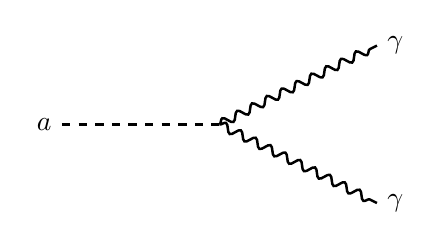
\begin{tikzpicture}[line width=0.9pt]
  \coordinate (a) at (-2.0, 0.0);
  \coordinate (v) at (0.0, 0.0);
  \coordinate (g1) at (2.0, 1.0);
  \coordinate (g2) at (2.0, -1.0);

  \node[left] at (a) {\(a\)};
  \node[right] at (g1) {\(\gamma\)};
  \node[right] at (g2) {\(\gamma\)};

  \draw[dashed] (a) -- (v);
  \draw[decorate, decoration={snake, amplitude=1.5pt, segment length=6pt}]
    (v) -- (g1);
  \draw[decorate, decoration={snake, amplitude=1.5pt, segment length=6pt}]
    (v) -- (g2);
\end{tikzpicture}
\caption{ALP decay to two photons, \(a\to\gamma\gamma\).}
\label{fig:alp-diphoton-decay}
\end{figure}

Since the center-of-mass frame of the ALP is boosted with respect to the lab
frame, the two photons do not generally have an angular separation
$\Delta\theta_{\gamma\gamma}=\pi$ in the detector. Instead, the opening angle
is a function of the ALP boost. Since calorimeters do not have arbitrarily
small angular resolution, if the angular separation of the photons is smaller
than the calorimeter resolution, the detector can register the two photons as
a single photon-like electromagnetic shower.

The vertex for the two-photon interaction is the same ALP--photon vertex used
in production,
\begin{equation}
    V^{\mu\nu}(k_1,k_2)
    =
    -ig_{a\gamma\gamma}\epsilon^{\mu\nu\alpha\beta}
    k_{1\alpha}k_{2\beta}.
    \label{eq:decay_vertex_repeat}
\end{equation}
Here $k_1$ and $k_2$ are the four-momenta of the two decay photons. Both
photons are outgoing, so the all-incoming vertex in Eq.~\eqref{eq:vertex} is
evaluated with momenta $-k_1$ and $-k_2$. The two minus signs cancel inside
the product $k_{1\alpha}k_{2\beta}$, so the vertex has the same momentum
dependence as before, up to an overall phase. The decay amplitude is obtained
by contracting the two photon indices of the vertex with the polarization
vectors of the two outgoing photons:
\begin{align}
    \mathcal{M}
    &=
    -iV^{\mu\nu}
    \varepsilon^{*}_{1\mu}(k_1)
    \varepsilon^{*}_{2\nu}(k_2)
    \nonumber\\
    &=
    -g_{a\gamma\gamma}\,
    \epsilon^{\mu\nu\alpha\beta}
    k_{1\alpha}k_{2\beta}
    \varepsilon^{*}_{1\mu}
    \varepsilon^{*}_{2\nu}.
    \label{eq:decay_amp}
\end{align}
The star denotes complex conjugation, as appropriate for outgoing external
particles. The polarization vectors $\varepsilon_1^\mu$ and
$\varepsilon_2^\nu$ describe the two physical transverse polarization states
of the photons. They should not be confused with the Levi-Civita symbol
$\epsilon^{\mu\nu\alpha\beta}$.

To compute a decay rate, we need the squared amplitude summed over the final
photon polarizations. It is useful to isolate the antisymmetric tensor carried
by the ALP--photon vertex,
\begin{equation}
    B_{\mu\nu}
    =
    \epsilon_{\mu\nu\alpha\beta}
    k_1^\alpha k_2^\beta,
    \qquad
    \mathcal{M}
    =
    -g_{a\gamma\gamma} B_{\mu\nu}
    \varepsilon_1^{*\mu}\varepsilon_2^{*\nu}.
    \label{eq:decay_tensor_form}
\end{equation}
The detector does not measure photon polarizations, so the observable decay
probability must include all allowed final polarization states. For a real
photon the physical polarizations are transverse,
$k\cdot\varepsilon^{(\lambda)}=0$, and the gauge-dependent terms in the
polarization sum vanish in this gauge-invariant amplitude. We can therefore
use
\begin{equation}
    \sum_{\lambda}
    \varepsilon_\mu^{(\lambda)*}(k)
    \varepsilon_{\mu'}^{(\lambda)}(k)
    \longrightarrow
    -g_{\mu\mu'}.
    \label{eq:photon_pol_sum}
\end{equation}
Applying this once for each outgoing photon gives
\begin{align}
    \sum_\mathrm{pol}|\mathcal{M}|^2
    &=
    g_{a\gamma\gamma}^2
    B_{\mu\nu}B_{\mu'\nu'}
    (-g^{\mu\mu'})(-g^{\nu\nu'})
    \nonumber\\
    &=
    g_{a\gamma\gamma}^2
    \epsilon^{\mu\nu\alpha\beta}
    \epsilon_{\mu\nu}^{\phantom{\mu\nu}\alpha'\beta'}
    k_{1\alpha}k_{2\beta}
    k_{1\alpha'}k_{2\beta'}.
    \label{eq:decay_m2_pol}
\end{align}
The remaining contraction uses the standard Levi-Civita identity
\begin{equation}
    \epsilon^{\mu\nu\alpha\beta}
    \epsilon_{\mu\nu}^{\phantom{\mu\nu}\alpha'\beta'}
    =
    -2\left(
      g^{\alpha\alpha'}g^{\beta\beta'}
      -
      g^{\alpha\beta'}g^{\beta\alpha'}
    \right).
    \label{eq:levicivita_contraction}
\end{equation}
Substituting this identity into Eq.~\eqref{eq:decay_m2_pol} gives
\begin{align}
    \sum_\mathrm{pol}|\mathcal{M}|^2
    &=
    -2g_{a\gamma\gamma}^2
    \left[
      (k_1\cdot k_1)(k_2\cdot k_2)
      -
      (k_1\cdot k_2)^2
    \right].
    \label{eq:decay_m2_step}
\end{align}
The photons are on shell and massless, so $k_1^2=k_2^2=0$. Thus the first term
vanishes, and
\begin{equation}
    \sum_\mathrm{pol}|\mathcal{M}|^2
    =
    2g_{a\gamma\gamma}^2(k_1\cdot k_2)^2.
    \label{eq:decay_m2_dot}
\end{equation}
Momentum conservation gives $p=k_1+k_2$, and the ALP is on shell with
$p^2=m_{a}^2$. Therefore
\begin{align}
    m_{a}^2
    &=
    (k_1+k_2)^2
    =
    k_1^2+2k_1\cdot k_2+k_2^2
    =
    2k_1\cdot k_2,
    \label{eq:k1k2_ma_relation}
\end{align}
or $k_1\cdot k_2=m_{a}^2/2$. Substituting this into
Eq.~\eqref{eq:decay_m2_dot} gives
\begin{equation}
    \sum_\mathrm{pol}|\mathcal{M}|^2
    =
    \frac{g_{a\gamma\gamma}^2m_{a}^4}{2}.
    \label{eq:decay_m2}
\end{equation}

There is no initial-state spin average in the decay because the ALP is a
spin-zero particle. For a two-body decay into identical massless particles,
\begin{equation}
    \Gamma
    =
    \frac{1}{2m_{a}}\frac{1}{2!}
    \int d\Phi_2\,\sum_\mathrm{pol}|\mathcal{M}|^2,
    \qquad
    \int d\Phi_2 = \frac{1}{8\pi}.
    \label{eq:decay_phase_space}
\end{equation}
The factor $1/(2m_{a})$ is the normalization for one decaying particle of mass
$m_{a}$. The factor $1/2!$ is needed because the two final photons are
identical: without it, the same physical final state would be counted twice
when the labels $1$ and $2$ are exchanged. Substituting
Eq.~\eqref{eq:decay_m2} gives
\begin{align}
    \Gamma(a\to\gamma\gamma)
    &=
    \frac{1}{2m_{a}}
    \frac{1}{2}
    \frac{1}{8\pi}
    \left(
      \frac{g_{a\gamma\gamma}^2m_{a}^4}{2}
    \right)
    \nonumber\\
    &=
    \frac{g_{a\gamma\gamma}^2m_{a}^3}{64\pi}.
    \label{eq:width_step}
\end{align}
This is the width used throughout the project:
\begin{equation}
    \Gamma(a\to\gamma\gamma)
    =
    \frac{g_{a\gamma\gamma}^2\,m_{a}^3}{64\pi}.
    \label{eq:width}
\end{equation}

For correctly paired photons from the ALP decay,
\begin{equation}
    M_{\gamma\gamma}^2=(k_1+k_2)^2
    =
    2E_1E_2(1-\cos\theta_{12})
    =
    m_{a}^2.
    \label{eq:mgg}
\end{equation}
Here $E_1$ and $E_2$ are the measured photon energies and $\theta_{12}$ is the
opening angle between the two photons. This invariant mass is independent of
the lab-frame boost of the ALP, so correctly paired decay photons form a peak
at $M_{\gamma\gamma}=m_{a}$. That peak is the main analysis observable in the
prompt-resolved channel.

The proper lifetime and proper decay length are
\begin{equation}
    \tau_a=\frac{1}{\Gamma_a},
    \qquad
    c\tau_a=\frac{\hbar c}{\Gamma_a},
    \label{eq:proper_lifetime}
\end{equation}
with $\hbar c=1.973269804\times10^{-16}\,\,\text{GeV}\,\mathrm{m}$. In the lab frame
the decay length is increased by the ALP boost,
\begin{equation}
    \ell_a
    =
    \beta_a\gamma_a c\tau_a
    =
    \frac{|\mathbf{p}_a|}{m_{a}}
    \frac{\hbar c}{\Gamma(a\to\gamma\gamma)}.
    \label{eq:lifetime}
\end{equation}
where $\beta_a=v_a/c$, $\gamma_a=E_a/m_{a}$, and
$\beta_a\gamma_a=|\mathbf{p}_a|/m_{a}$. Equations~\eqref{eq:width}
and~\eqref{eq:lifetime} show that $\ell_a$ decreases with increasing
$g_{a\gamma\gamma}$ and increasing $m_{a}$: heavy, strongly coupled ALPs decay promptly,
while light, weakly coupled ALPs are long-lived and escape the detector.

The probability density for an ALP to decay after travelling a lab-frame
distance $L$ is exponential,
\begin{equation}
    f(L)=\frac{1}{\ell_a}e^{-L/\ell_a}.
\end{equation}
Integrating this density over the relevant detector length intervals gives the
probabilities used in the analytic scan:
\begin{align}
    P(L>L_\mathrm{max})
    &=
    e^{-L_\mathrm{max}/\ell_a},
    \label{eq:survival_prob}\\
    P(L<L_\mathrm{min})
    &=
    1-e^{-L_\mathrm{min}/\ell_a},\\
    P(L_\mathrm{min}<L<L_\mathrm{max})
    &=
    e^{-L_\mathrm{min}/\ell_a}
    -
    e^{-L_\mathrm{max}/\ell_a}.
    \label{eq:decay_window_prob}
\end{align}
The first line is the survival probability to the outer detector radius
$L_\mathrm{max}$ and defines the invisible signature. The second is the
probability to decay before the prompt-distance scale $L_\mathrm{min}$. The
third is the probability to decay between those two scales, producing a
displaced signature.

The angular resolution boundary follows from boosting the isotropic
$a\to\gamma\gamma$ decay. For an ALP moving along the $z$ axis, the two photons
are emitted back-to-back in the ALP rest frame. The smallest lab-frame opening
angle occurs when the rest-frame photons are emitted transverse to the boost,
for which
\begin{equation}
    \Delta\theta_{\gamma\gamma}^{\min}
    =
    2\arctan\!\left(\frac{1}{\gamma_a\beta_a}\right)
    =
    2\arctan\!\left(\frac{m_{a}}{|\mathbf{p}_a|}\right).
    \label{eq:dtheta_exact}
\end{equation}
The physical reason is simple: a highly boosted ALP carries the two decay
photons forward in almost the same direction, so the two electromagnetic
showers can merge in the calorimeter. For light ALPs,
$|\mathbf{p}_a|\simeq\sqrt{s}/2$ and $\gamma_a\simeq\sqrt{s}/(2m_{a})$, so
\begin{equation}
    \Delta\theta_{\gamma\gamma}^{\min}
    \simeq
    \frac{2}{\gamma_a}
    \simeq
    \frac{4m_{a}}{\sqrt{s}}.
    \label{eq:dtheta}
\end{equation}
The prompt-resolved channel requires this opening angle to be larger than the
detector angular resolution, $\Delta\theta_\mathrm{res}$. If
$\Delta\theta_{\gamma\gamma}^{\min}<\Delta\theta_\mathrm{res}$, the two photons
are treated as merged even if the ALP decays promptly.

\subsection{Detector-level signal categories}

The ALP phenomenology at the detector level is therefore determined by two
parameters: the decay length $\ell_a$ and the minimum diphoton opening angle
$\Delta\theta^{\mathrm{min}}_{\gamma\gamma}$ of the ALP decay products. We can
therefore classify each point $(m_{a},g_{a\gamma\gamma})$ in parameter space into four
exclusive signatures:
\begin{enumerate}
    \item \textbf{Invisible $(\ell_a>L_\mathrm{max})$:}
    The ALP escapes the detector before decaying, leaving only a single photon
    $\gamma_{\mathrm{recoil}}$ with missing energy as signature,
    $e^+e^-\to\gamma_{\mathrm{recoil}}+\not\!E$.

    \item \textbf{Prompt-resolved $(\ell_a<L_{\mathrm{min}}$ and
    $\Delta\theta^\mathrm{min}_{\gamma\gamma}\geq\Delta\theta_\mathrm{res})$:}
    The ALP decays immediately into two resolvable photons,
    $e^+e^-\to\gamma_{\mathrm{recoil}}+\gamma\gamma$. The three-photon final
    state carries an invariant-mass peak at $m_{a}$.

    \item \textbf{Displaced-resolved
    $(L_{\mathrm{min}}\leq \ell_a \leq L_{\mathrm{max}})$:}
    The ALP decays inside the detector but away from the interaction point.

    \item \textbf{Merged $(\ell_a<L_{\mathrm{max}}$ and
    $\Delta\theta^\mathrm{min}_{\gamma\gamma}<\Delta\theta_\mathrm{res})$:}
    The decay photons cannot be angularly resolved, so the signal resembles a
    single photon.
\end{enumerate}

In this analysis we focus on the invisible and prompt-resolved signatures. We
make this choice because the displaced-resolved and merged signatures require
more precise detector and background modeling, which is beyond the scope of
this project, while the invisible and prompt-resolved signatures give a clean
first projection. The decay width, decay length, decay probabilities, and
angular separation derived above are the quantities used to make this
classification quantitative.

% ============================================================
\section{Simulation and Detector Modeling}
\label{sec:simulation}

\subsection{Simulation strategy}

The analysis is a counting problem repeated over the
$(m_{a},g_{a\gamma\gamma})$ plane. For each point we ask two things. First:
what kind of event would an ALP make in the detector? Second: would that event
be large enough compared with the Standard Model background to be excluded?
The first question is mostly analytic. The second needs simulation.

The basic event yield is
\begin{equation}
    N = \sigma\,\mathcal{L},
    \label{eq:basic_yield}
\end{equation}
where $\sigma$ is the cross section and $\mathcal{L}$ is the integrated
luminosity. For the FCC-ee Z-pole run we use
$\mathcal{L}=150\,\text{ab}^{-1}=1.5\times10^8\,\text{pb}^{-1}$, so even very
small cross sections can give visible event counts. But Eq.~\eqref{eq:basic_yield}
is not yet what the detector sees. A produced event still has to decay in the
right part of the detector, pass the photon acceptance, be reconstructed, and
fall into the analysis histogram. This is why we use
\begin{equation}
    N_\mathrm{sig}
    =
    \mathcal{L}\,
    \sigma(m_{a},g_{a\gamma\gamma})\,
    P_\mathrm{region}(m_{a},g_{a\gamma\gamma})\,
    \epsilon_\mathrm{param}\,
    C_\mathrm{Delphes}.
    \label{eq:nsig}
\end{equation}
Here $P_\mathrm{region}$ is the probability that the ALP is in the signal
region, $\epsilon_\mathrm{param}$ is the simple photon acceptance and
reconstruction efficiency, and $C_\mathrm{Delphes}$ is the correction measured
from detector-level simulation.

This is the central logic of the project. The analytic formulas tell us where
the ALP decays, what the recoil energy is, and how the yield scales with
$g_{a\gamma\gamma}$. Delphes tells us what survives as reconstructed photons.
The Standard Model simulation tells us how much background sits under the same
observable. The exclusion contour is then the place where the expected signal
equals the signal required to stand out from that background.

We do not run the full detector simulation at every grid point. That would be
slow and mostly unnecessary, because for associated production
$\sigma(e^+e^-\to\gamma a)\propto g_{a\gamma\gamma}^2$ exactly at tree level.
So the dense scan is analytic, while the full
MadGraph--Pythia--Delphes chain is used to validate and correct it. The final
inputs are:
\begin{itemize}
    \item an analytic grid of $180\times180=32\,400$ points;
    \item 284 detector-level ALP signal points, each with $10\,000$ events;
    \item one $e^+e^-\to\gamma\gamma\gamma$ background sample with
    $10\,000$ events;
    \item one $e^+e^-\to\gamma\nu\bar{\nu}$ background sample with
    $10\,000$ events.
\end{itemize}
The generated Monte Carlo event counts are not the FCC-ee event counts. They
are finite samples used to estimate shapes, efficiencies, and checks. The
physical normalization always comes from the MadGraph cross section multiplied
by the FCC-ee luminosity.

\subsection{Scan ranges and model choices}

The final FCC-ee projection is evaluated on a logarithmic
$180\times180$ grid,
\begin{equation}
    m_{a} \in [10^{-2},80]\,\text{GeV},
    \qquad
    g_{a\gamma\gamma} \in [10^{-8},10^{-1}]\,\text{GeV}^{-1}.
    \label{eq:scan_range}
\end{equation}
The lower mass bound is chosen because below about $10\,\text{MeV}$ the two
photons from $a\to\gamma\gamma$ are too collimated to be resolved at the
Z pole for the angular resolution used here. The upper mass bound is chosen
because associated production is strongly suppressed close to the kinematic
endpoint, through the factor $(1-m_{a}^2/s)^3$. The upper value
$80\,\text{GeV}$ still keeps the high-mass collider region, but avoids turning
the result into a threshold study. The coupling range is wide on purpose. The
lower end is below the event-yield floor at $150\,\text{ab}^{-1}$, while the
upper end brackets the lifetime boundary where the ALP decays before it can
escape the detector. The very large coupling end is therefore a numerical
bracket, not a claim that every point is a controlled EFT benchmark.

We focus on the FCC-ee Z-pole run because it has the largest projected
luminosity, about $150\,\text{ab}^{-1}$, and therefore gives the cleanest first
benchmark for a rare process. The FCC-ee will also run at higher energies, but
those stages have smaller luminosities and would require separately optimized
searches. In this project the Z pole is used only as a high-luminosity
$e^+e^-$ collider environment. We do not use resonant $Z\to\gamma a$
production. Instead, we keep the photophilic benchmark in which the ALP couples
to photons and is produced by ALP-strahlung,
$e^+e^-\to\gamma^\ast\to\gamma a$.

There is one technical point in connecting this physical benchmark to the UFO
model. The imported UFO does not expose $g_{a\gamma\gamma}$ directly. It uses
the internal parameters $f_a$, $K_B$, and $K_W$, which are related to the
physical coupling by
\begin{equation}
    g_{a\gamma\gamma}=
    \frac{\alpha_\mathrm{em}(K_B+K_W)}
    {\sqrt{2}\,\pi f_a}.
    \label{eq:ufo_mapping}
\end{equation}
In the scan we fix $f_a=1000\,\text{GeV}$ and vary the dimensionless sum
$K_B+K_W$ to obtain the requested value of $g_{a\gamma\gamma}$. This is only a
coordinate choice inside the UFO. The reported result is always in the
physical $(m_{a},g_{a\gamma\gamma})$ plane. With this choice,
\begin{equation}
    K_B+K_W
    =
    \frac{\sqrt{2}\,\pi f_a}{\alpha_\mathrm{em}}g_{a\gamma\gamma}
    =
    6.09\times10^{5}
    \left(\frac{g_{a\gamma\gamma}}{\text{GeV}^{-1}}\right).
    \label{eq:k_sum_numeric}
\end{equation}
Therefore the grid
$g_{a\gamma\gamma}\in[10^{-8},10^{-1}]\,\text{GeV}^{-1}$ corresponds internally
to
\begin{equation}
    K_B+K_W\in[6.09\times10^{-3},\,6.09\times10^{4}].
    \label{eq:k_sum_range}
\end{equation}
The upper end is only used to bracket the short-lifetime boundary, and should
not be interpreted as a statement that every point is a perturbative EFT model.

The UFO also contains an $a\gamma Z$ vertex. In the model this coupling is
proportional to
\begin{equation}
    C_{\gamma Z}\propto K_W c_w^2-K_B s_w^2,
    \label{eq:cgz}
\end{equation}
where $s_w$ and $c_w$ are computed from the same electroweak inputs as the UFO.
To remove the tree-level ALP--$Z$ coupling while keeping the desired
$a\gamma\gamma$ coupling, the parameter-card writer uses
\begin{equation}
    K_B=(K_B+K_W)c_w^2,
    \qquad
    K_W=(K_B+K_W)s_w^2.
    \label{eq:photophilic_split}
\end{equation}
This makes Eq.~\eqref{eq:cgz} vanish at tree level. Numerically, with the
electroweak inputs used by the UFO, $s_w^2=0.212154$ and
$c_w^2=0.787846$, so the code sets
$K_B=0.787846(K_B+K_W)$ and $K_W=0.212154(K_B+K_W)$ for every generated point.
This is important because otherwise the Z-pole result would mix two different
questions: photophilic ALP-strahlung and resonant $Z\to\gamma a$ production.

\subsection{MadGraph}

The detector-level chain for one signal point is:
\begin{equation}
    \begin{aligned}
    \texttt{param\_card}
    &\to \textsc{MadGraph}\;(\text{LHE})
    \to \textsc{Pythia}\;(\text{HepMC})\\
    &\to \textsc{Delphes}\;(\text{ROOT})
    \to \text{Python validation}.
    \end{aligned}
    \label{eq:pipeline}
\end{equation}
MadGraph is the first simulation step. It takes the UFO model, the beam energy,
the process definition, and the parameter card for one
$(m_{a},g_{a\gamma\gamma})$ point. For the signal the process is
$e^+e^-\to\gamma a$. MadGraph computes the matrix element, integrates the
phase space, reports the production cross section, and writes an LHE event
file. The LHE file is still a generator-level file: it contains the hard
scattering particles and momenta, but it does not yet contain the detector
response.

The same MadGraph step is also used for the Standard Model backgrounds. The
resolved-prompt background is $e^+e^-\to\gamma\gamma\gamma$, and the invisible
background is $e^+e^-\to\gamma\nu\bar{\nu}$. These backgrounds are generated
separately from the signal because the background does not depend on
$m_{a}$ or $g_{a\gamma\gamma}$. Once the background shapes are made, they can
be reused for every ALP point.

\subsection{MadGraph verification}

The first validation is a cross-section check. MadGraph must reproduce the
analytic associated-production result,
\begin{equation}
    \sigma(e^+e^-\to\gamma a)
    =
    \frac{\alpha g_{a\gamma\gamma}^2}{12}
    \left(1-\frac{m_{a}^{2}}{s}\right)^3,
    \label{eq:mg_verification_xsec}
\end{equation}
after converting from $\text{GeV}^{-2}$ to pb. This test checks that the UFO
coupling, the process definition, the beam setup, and the parameter-card
mapping are all consistent with the analytic convention used in the theory
section. In the full FCC-ee signal campaign all 284 detector-level ALP points
passed this Gate 1 check. A separate Standard Model
$e^+e^-\to\mu^+\mu^-$ smoke test was also used before the ALP scan, because it
is a simple way to check that MadGraph produces sensible $e^+e^-$ events at
the chosen center-of-mass energy.

\subsection{Pythia}

Pythia reads the LHE file from MadGraph. In this project it is used for two
things. First, it adds QED radiation to the event record. Second, for the full
ALP detector-level samples, it decays the ALP to two photons with the physical
lifetime. The lifetime is obtained from the width
\begin{equation}
    \Gamma(a\to\gamma\gamma)
    =
    \frac{g_{a\gamma\gamma}^2m_{a}^3}{64\pi}.
    \label{eq:pythia_width}
\end{equation}
Pythia needs the lifetime in millimeters, while the analytic calculation uses
meters, so this is a place where a unit mistake would immediately change the
signature classification. After Pythia, the event is written as a HepMC file,
which is the format passed to Delphes.

\subsection{Pythia verification}

The Pythia validation checks the width and lifetime convention. The project
uses the $64\pi$ convention in Eq.~\eqref{eq:pythia_width}, and the parameter
card writer uses the same convention when it writes the ALP width. The Pythia
stage then checks that the decay length implied by the event record is
consistent with the analytic boosted decay length,
\begin{equation}
    \ell_a=\frac{|\mathbf{p}_a|}{m_{a}}\frac{\hbar c}{\Gamma_a}.
    \label{eq:pythia_decay_length_check}
\end{equation}
This is Gate 2. It matters because the invisible and prompt-resolved contours
are lifetime boundaries as much as cross-section boundaries. If the ALP
lifetime were off by a factor of two, the invisible and prompt regions would
move in the $(m_{a},g_{a\gamma\gamma})$ plane.

\subsection{Delphes}

Delphes is not a full detector simulation, but it is enough for this project
because we need the main reconstruction effects: acceptance, photon efficiency,
energy smearing, object counting, and missing energy. The locked detector
numbers are:
\begin{itemize}
    \item Photon acceptance: $|\eta| < 3.0$, $E_\gamma > 0.5\,\text{GeV}$;
    \item Photon reconstruction efficiency: 99\%;
    \item Diphoton angular resolution: $\Delta\theta_\mathrm{res} = 1.5^\circ$
    (conservative calorimeter-cell scale, $\pi/120$);
    \item Tracker inner radius ($L_\mathrm{min}$): $0.02\,\text{m}$;
    \item Tracker/calorimeter outer radius ($L_\mathrm{max}$): $2.5\,\text{m}$.
\end{itemize}

For the FCC-ee projection we use an IDEA-like Delphes card. The Delphes output
is a ROOT file with reconstructed objects such as photons and missing
transverse energy. The Python analysis then reads these ROOT files with
\texttt{uproot}, forms the diphoton invariant mass for the prompt-resolved
channel, and forms the recoil-photon energy for the invisible channel.

The background samples are passed through the same MadGraph--Pythia--Delphes
chain at $\sqrt{s}=91.2\,\text{GeV}$. Two channels are generated:
\begin{itemize}
    \item \textbf{Resolved-prompt background}: $e^+e^-\to\gamma\gamma\gamma$
    (SM QED triple-photon production),
    with $\sigma = 7.306\,\text{pb}$ and $N_\mathrm{gen} = 10\,000$ events.
    After Delphes and object selection, the resolved histogram contains
    23\,592 diphoton-pair entries. This number can be larger than the number of
    selected events because one event with several photons contributes several
    photon pairs.

    \item \textbf{Invisible background}: $e^+e^-\to\gamma\nu\bar{\nu}$
    (radiative neutrino production),
    with $\sigma = 134.9\,\text{pb}$ and $N_\mathrm{gen} = 10\,000$ events.
    After Delphes and the exactly-one-photon selection, the recoil-energy
    histogram contains 2\,684 entries.
\end{itemize}
The backgrounds are generated separately from the signal. This is much more
practical than generating a new mixed sample for every possible ALP mass and
coupling. For the limit, each background histogram is normalized to the FCC-ee
luminosity,
\begin{equation}
    B_i
    =
    n_i^\mathrm{raw}
    \frac{\sigma_\mathrm{bkg}\,\mathcal{L}}{N_\mathrm{gen}},
    \label{eq:bkg_norm}
\end{equation}
where $n_i^\mathrm{raw}$ is the raw bin count in the Monte Carlo sample. The
background does not change the ALP lifetime or topology. It only changes the
number of signal events needed to claim sensitivity.

\subsection{Delphes verification}

The Delphes verification checks that the detector-level ROOT files contain the
objects needed by the analysis and that the reconstructed observables peak in
the expected places. For prompt-resolved ALP events, the relevant object is the
best reconstructed photon pair in events with at least three photons. Its
invariant mass must peak near the generated $m_{a}$. For invisible events, the
recoil-photon energy must peak near the two-body value
$E_\gamma=(s-m_{a}^{2})/(2\sqrt{s})$. In the full channel-aware campaign, all
284 detector-level signal points passed the detector validation and were used
to build the correction map $C_\mathrm{Delphes}$ in Eq.~\eqref{eq:nsig}.

\begin{figure}[H]
    \centering
    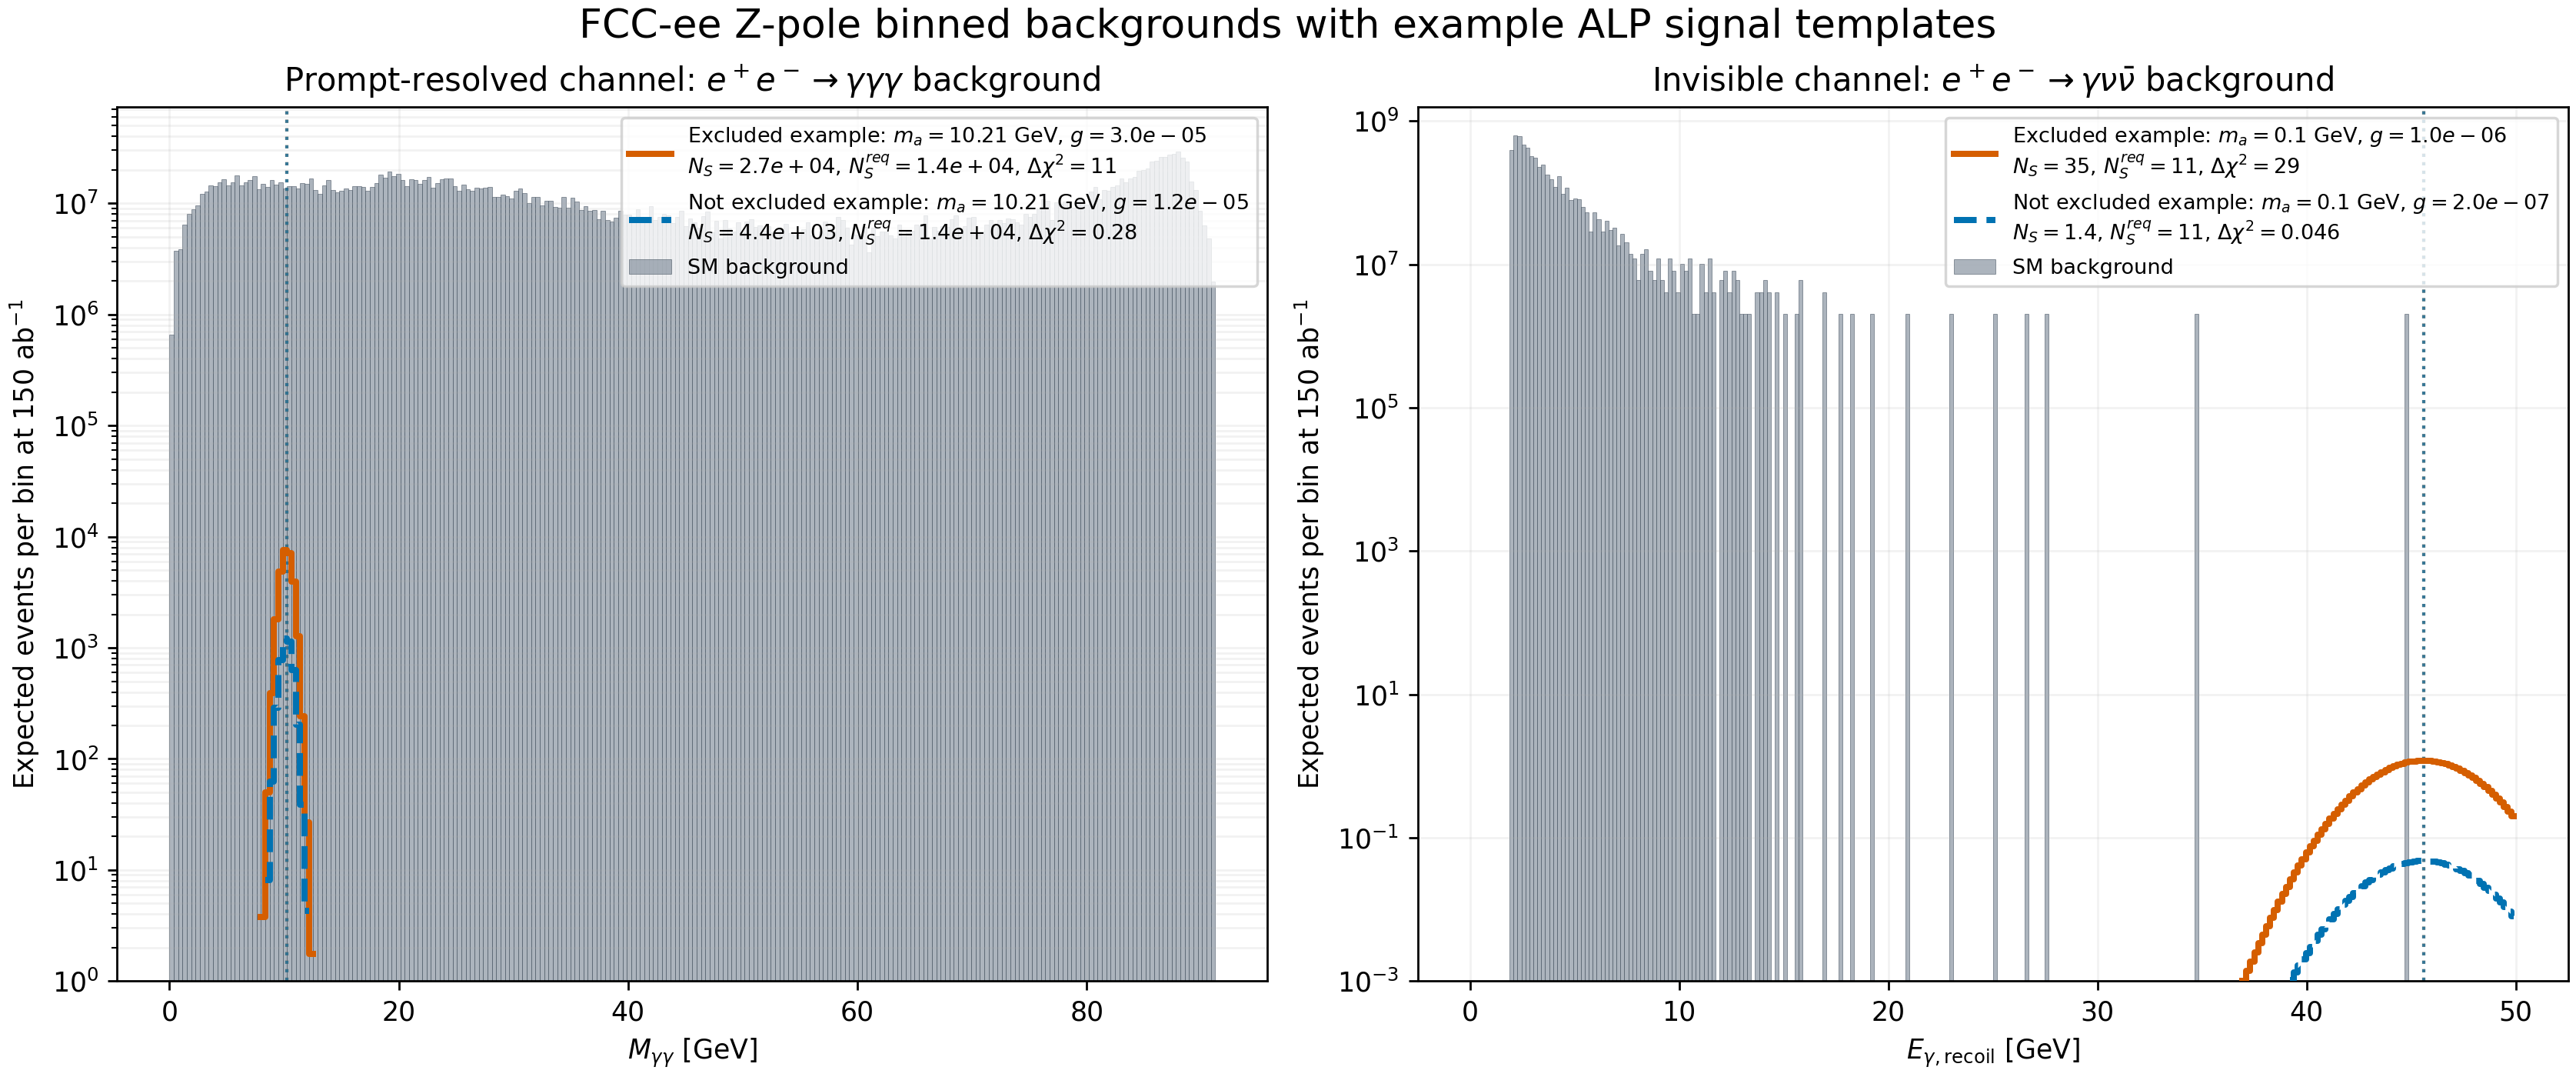
\includegraphics[width=\textwidth]{figures/background_signal_examples.png}
    \caption{Background histograms used in the FCC-ee limit calculation, with
    example ALP signals overlaid. The resolved channel uses
    $M_{\gamma\gamma}$, while the invisible channel uses recoil-photon energy.}
    \label{fig:background_signal_examples}
\end{figure}

\begin{figure}[H]
    \centering
    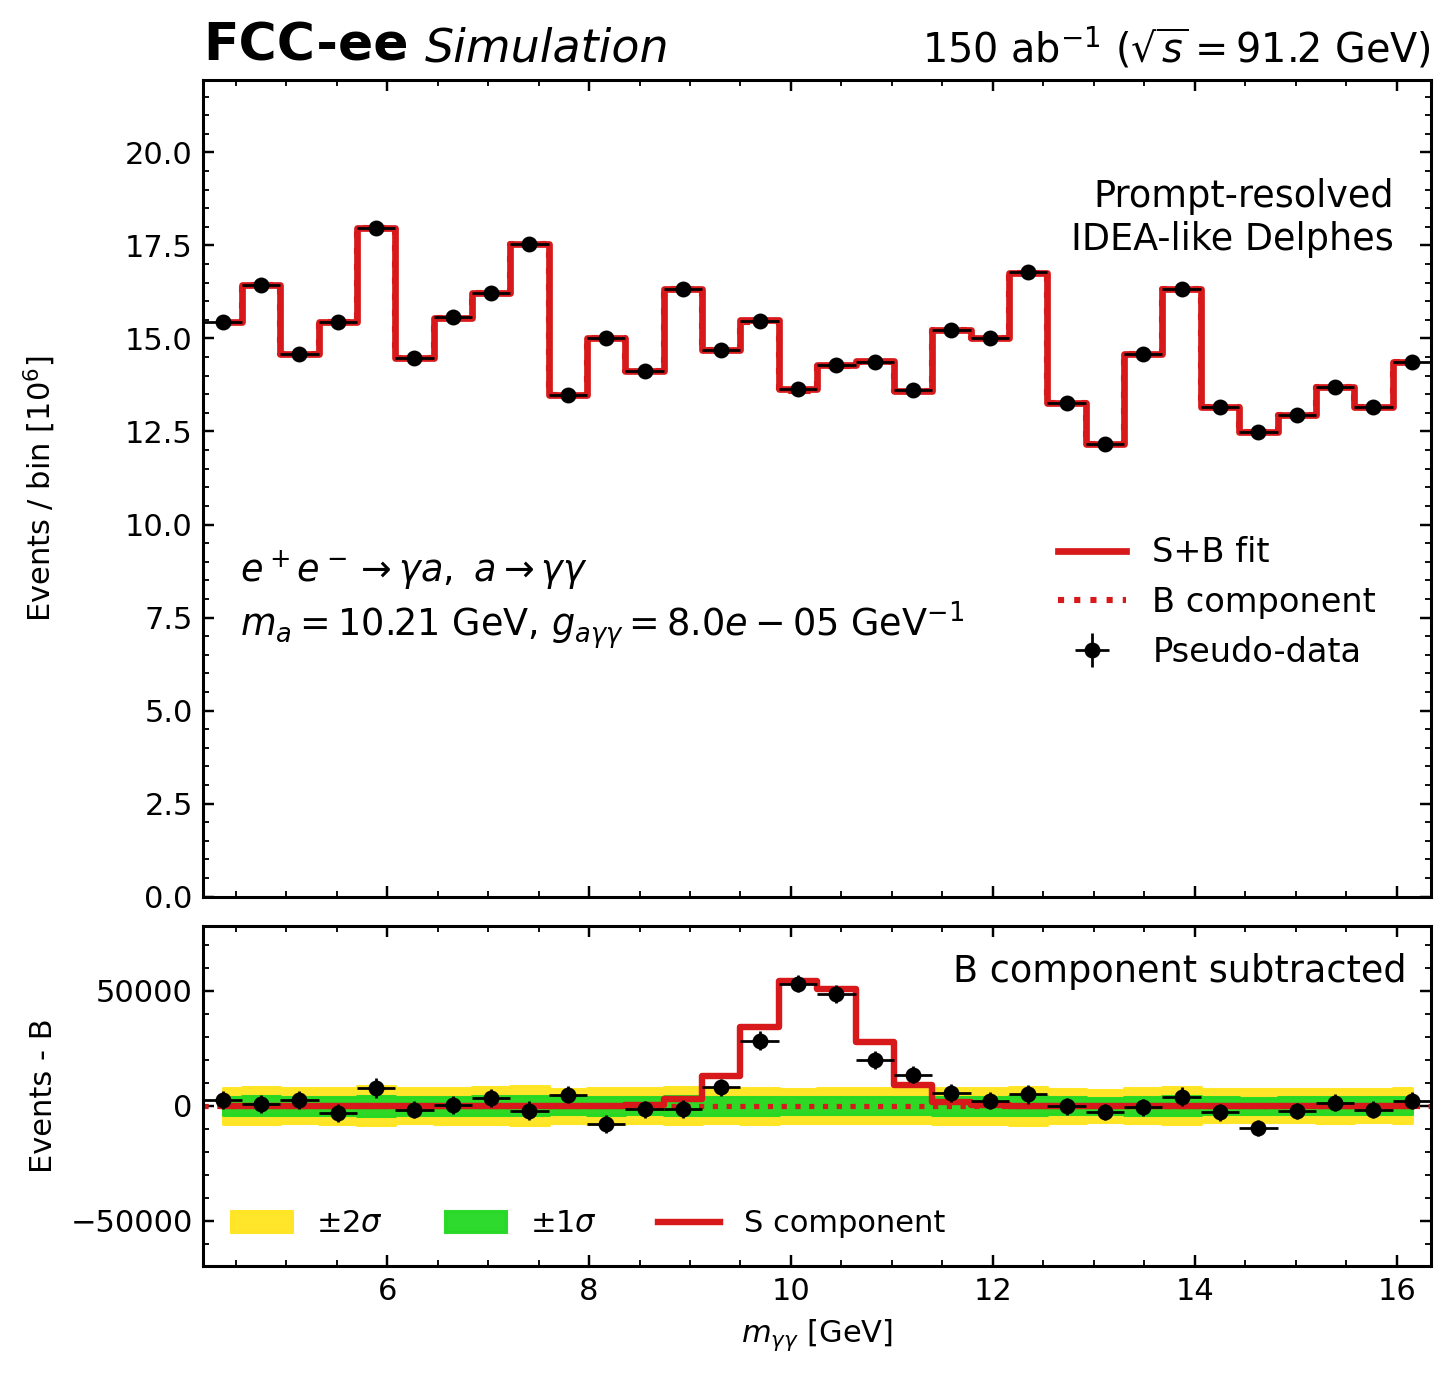
\includegraphics[width=0.92\textwidth]{figures/prompt_resolved_invariant_mass_example.png}
    \caption{Prompt-resolved invariant-mass verification plot for one example
    ALP point, $m_{a}=10.21\,\text{GeV}$ and
    $g_{a\gamma\gamma}=8.0\times10^{-5}\,\text{GeV}^{-1}$. The top panel shows
    pseudo-data, the Standard Model background template, and the
    signal-plus-background template. The lower panel subtracts the background,
    making the reconstructed ALP peak visible relative to the expected
    background fluctuations.}
    \label{fig:prompt_resolved_mass_verification}
\end{figure}

\subsection{Belle II closure test}

The final validation is the Belle~II closure test. This is different from the
previous checks because it tests the physics interpretation, not just whether
the software chain runs. The code loads the public Belle~II contour from
AxionLimits, converts it to the same units, applies the same analytic
production, lifetime, acceptance, and prompt-resolved logic used later for
FCC-ee, and checks whether the contour can be reconstructed. The maximum
residual is
\begin{equation}
    \max_{m_{a}}
    \left|\log_{10}\!\left(\frac{g_\mathrm{closure}}{g_\mathrm{published}}\right)\right|
    = 7.6\times10^{-3},
    \label{eq:closure}
\end{equation}
so the public-contour closure passes well within the 2\% tolerance.

\begin{figure}[H]
    \centering
    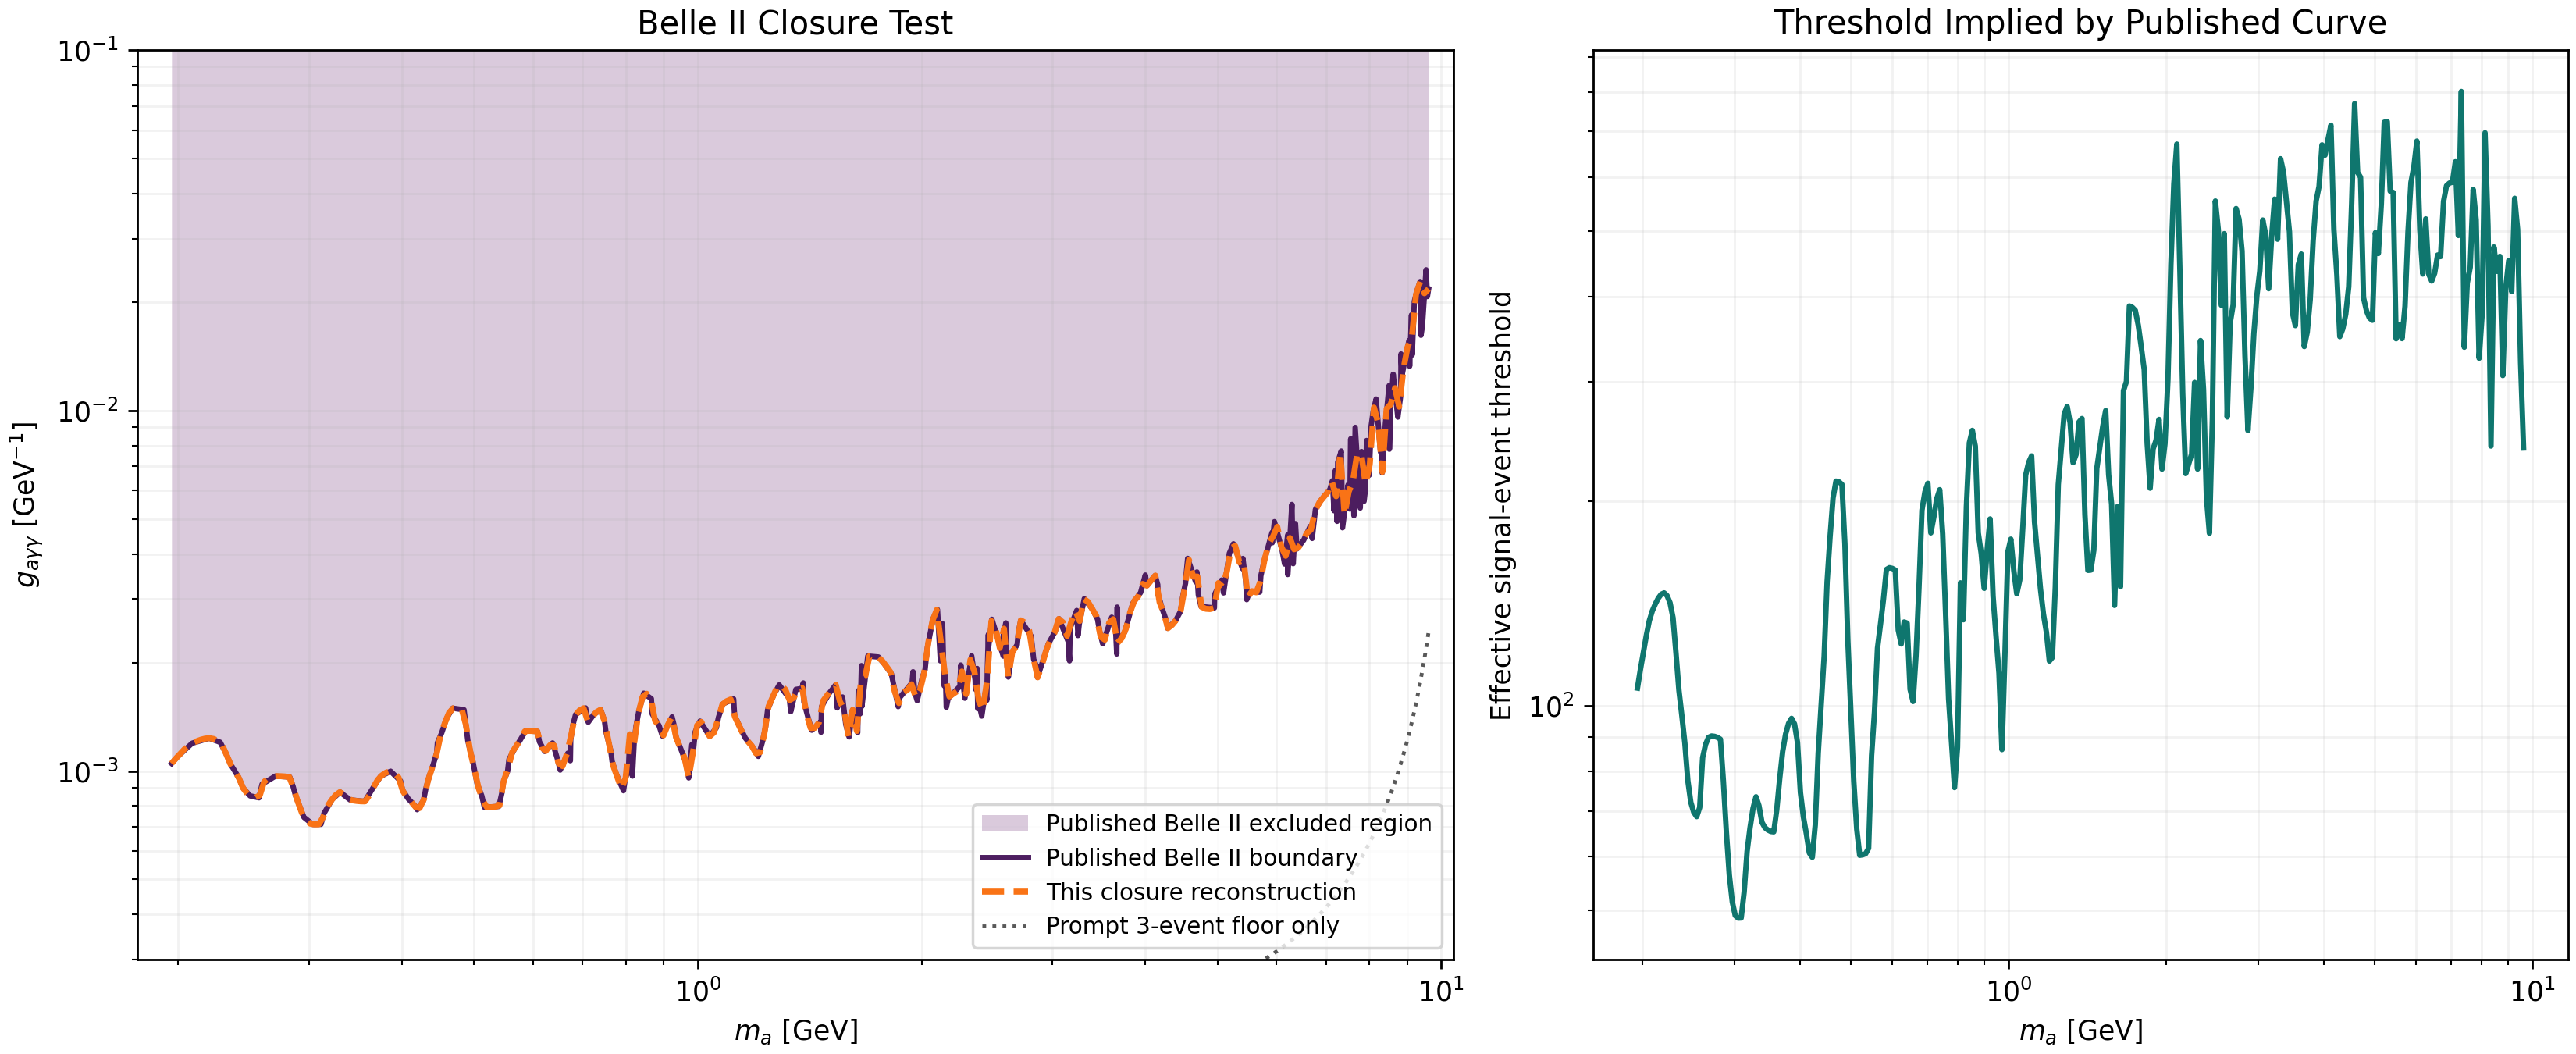
\includegraphics[width=\textwidth]{figures/belle2_closure.png}
    \caption{Belle~II public-contour closure test. The reconstructed contour
    agrees with the published Belle~II boundary, which checks the cross-section,
    lifetime, acceptance, and prompt-resolved logic used later for FCC-ee.}
    \label{fig:belle2_closure}
\end{figure}

% ============================================================
\section{Analysis}
\label{sec:analysis}

\subsection{Signature classification and efficiency}

Each of the $180\times180 = 32\,400$ grid points $(m_{a}, g_{a\gamma\gamma})$ is
classified as invisible, prompt-resolved, displaced-resolved, or merged. This
is not yet an exclusion limit. It is just the map of what kind of signal the
detector would see. The code compares the decay length $\ell_a$ with
$L_\mathrm{min}$ and $L_\mathrm{max}$, and compares the photon opening angle
with $\Delta\theta_\mathrm{res}$. The prompt-resolved threshold mass is set by
$\Delta\theta_\mathrm{min} = \Delta\theta_\mathrm{res}$:
\begin{equation}
    m_{a}^\mathrm{thresh} = \frac{\sqrt{s}\,\Delta\theta_\mathrm{res}}{4}
    \approx \frac{91.2\,\text{GeV} \times 0.0262}{4} \approx 0.597\,\text{GeV}.
    \label{eq:threshold}
\end{equation}
Below this value the photons are merged. Above it, prompt decays can be used in
the resolved three-photon search.

The lifetime probabilities used in Eq.~\eqref{eq:nsig} are
\begin{align}
    P_\mathrm{invisible} &= e^{-L_\mathrm{max}/\ell_a},
    \label{eq:pinv}\\
    P_\mathrm{prompt} &= 1 - e^{-L_\mathrm{min}/\ell_a}.
    \label{eq:pprompt}
\end{align}
The detector correction is obtained from the 284 full signal points. These
points were chosen on the contour-relevant branches: the lower invisible
branch, the upper invisible lifetime branch, and the prompt-resolved branch.
For each point the analysis counts how many generated signal events become
usable reconstructed events. The ratio to the analytic efficiency is
\begin{equation}
    C_\mathrm{Delphes}
    =
    \frac{
      f_\mathrm{selected}^\mathrm{Delphes}
    }{
      P_\mathrm{region}\epsilon_\mathrm{param}
    }.
    \label{eq:delphes_correction}
\end{equation}
This correction is then interpolated branch by branch and put back into
Eq.~\eqref{eq:nsig}. The prompt-resolved and lower invisible branches have
corrections close to one. The upper invisible branch is less stable because it
lies on a steep lifetime boundary, where small changes in lifetime produce very
large changes in survival probability.

\subsection{Limit-setting method}

A projected 90\% confidence level exclusion is calculated with a binned Asimov
$\Delta\chi^2$ test~\cite{Cowan2011}. ``Asimov'' means that the expected data
are assumed to be exactly the Standard Model background. So the question is:
if FCC-ee saw no excess, what ALP signal would be large enough to exclude?

The resolved channel uses the diphoton invariant mass $M_{\gamma\gamma}$, with
a Gaussian signal peak centered at $m_{a}$. The invisible channel uses the
recoil photon energy, with a Gaussian peak centered at
$E_\gamma=(s-m_{a}^2)/(2\sqrt{s})$. In both cases the signal template is written
as bin fractions $f_i$, while the background expectation in each bin is $B_i$.

With background-only Asimov data, the binned test statistic reduces to
\begin{equation}
    \Delta\chi^2(N_\mathrm{sig})
    =
    \sum_i
    \frac{(N_\mathrm{sig} f_i)^2}{\max(B_i,1)}.
    \label{eq:binned_dchi}
\end{equation}
The denominator uses $\max(B_i,1)$ so that empty Monte Carlo bins do not give
infinite sensitivity. Solving $\Delta\chi^2=2.71$ gives the required signal
count:
\begin{equation}
    N_\mathrm{sig}^\mathrm{req} =
    \max\!\left(3,\;
    \sqrt{\frac{2.71}{\displaystyle\sum_i f_i^2 / \max(B_i, 1)}}
    \right),
    \label{eq:nsig_req}
\end{equation}
The factor of 3 is a conservative minimum-event floor. The contour is then
found by solving
\begin{equation}
    N_\mathrm{sig}(m_{a},g_{a\gamma\gamma})
    =
    N_\mathrm{sig}^\mathrm{req}(m_{a})
    \label{eq:contour_condition}
\end{equation}
at each mass. If the expected signal is above the required signal, that point
would be excluded in the projected background-only FCC-ee dataset. The
invisible contour has two branches because its yield is non-monotonic in
$g_{a\gamma\gamma}$: at small coupling too few ALPs are produced, while at large
coupling the ALP decays before escaping.

% ============================================================
\section{Results}
\label{sec:results}

Figure~\ref{fig:classification} shows the topology map. The invisible region
dominates at low coupling, the prompt-resolved region appears at higher
coupling above the angular-resolution threshold, the merged region sits at low
mass where the two photons are too close, and the displaced region is the
transition between prompt and invisible. This is useful because it tells us
which analysis should be used before we make the exclusion contour.

\begin{figure}[H]
    \centering
    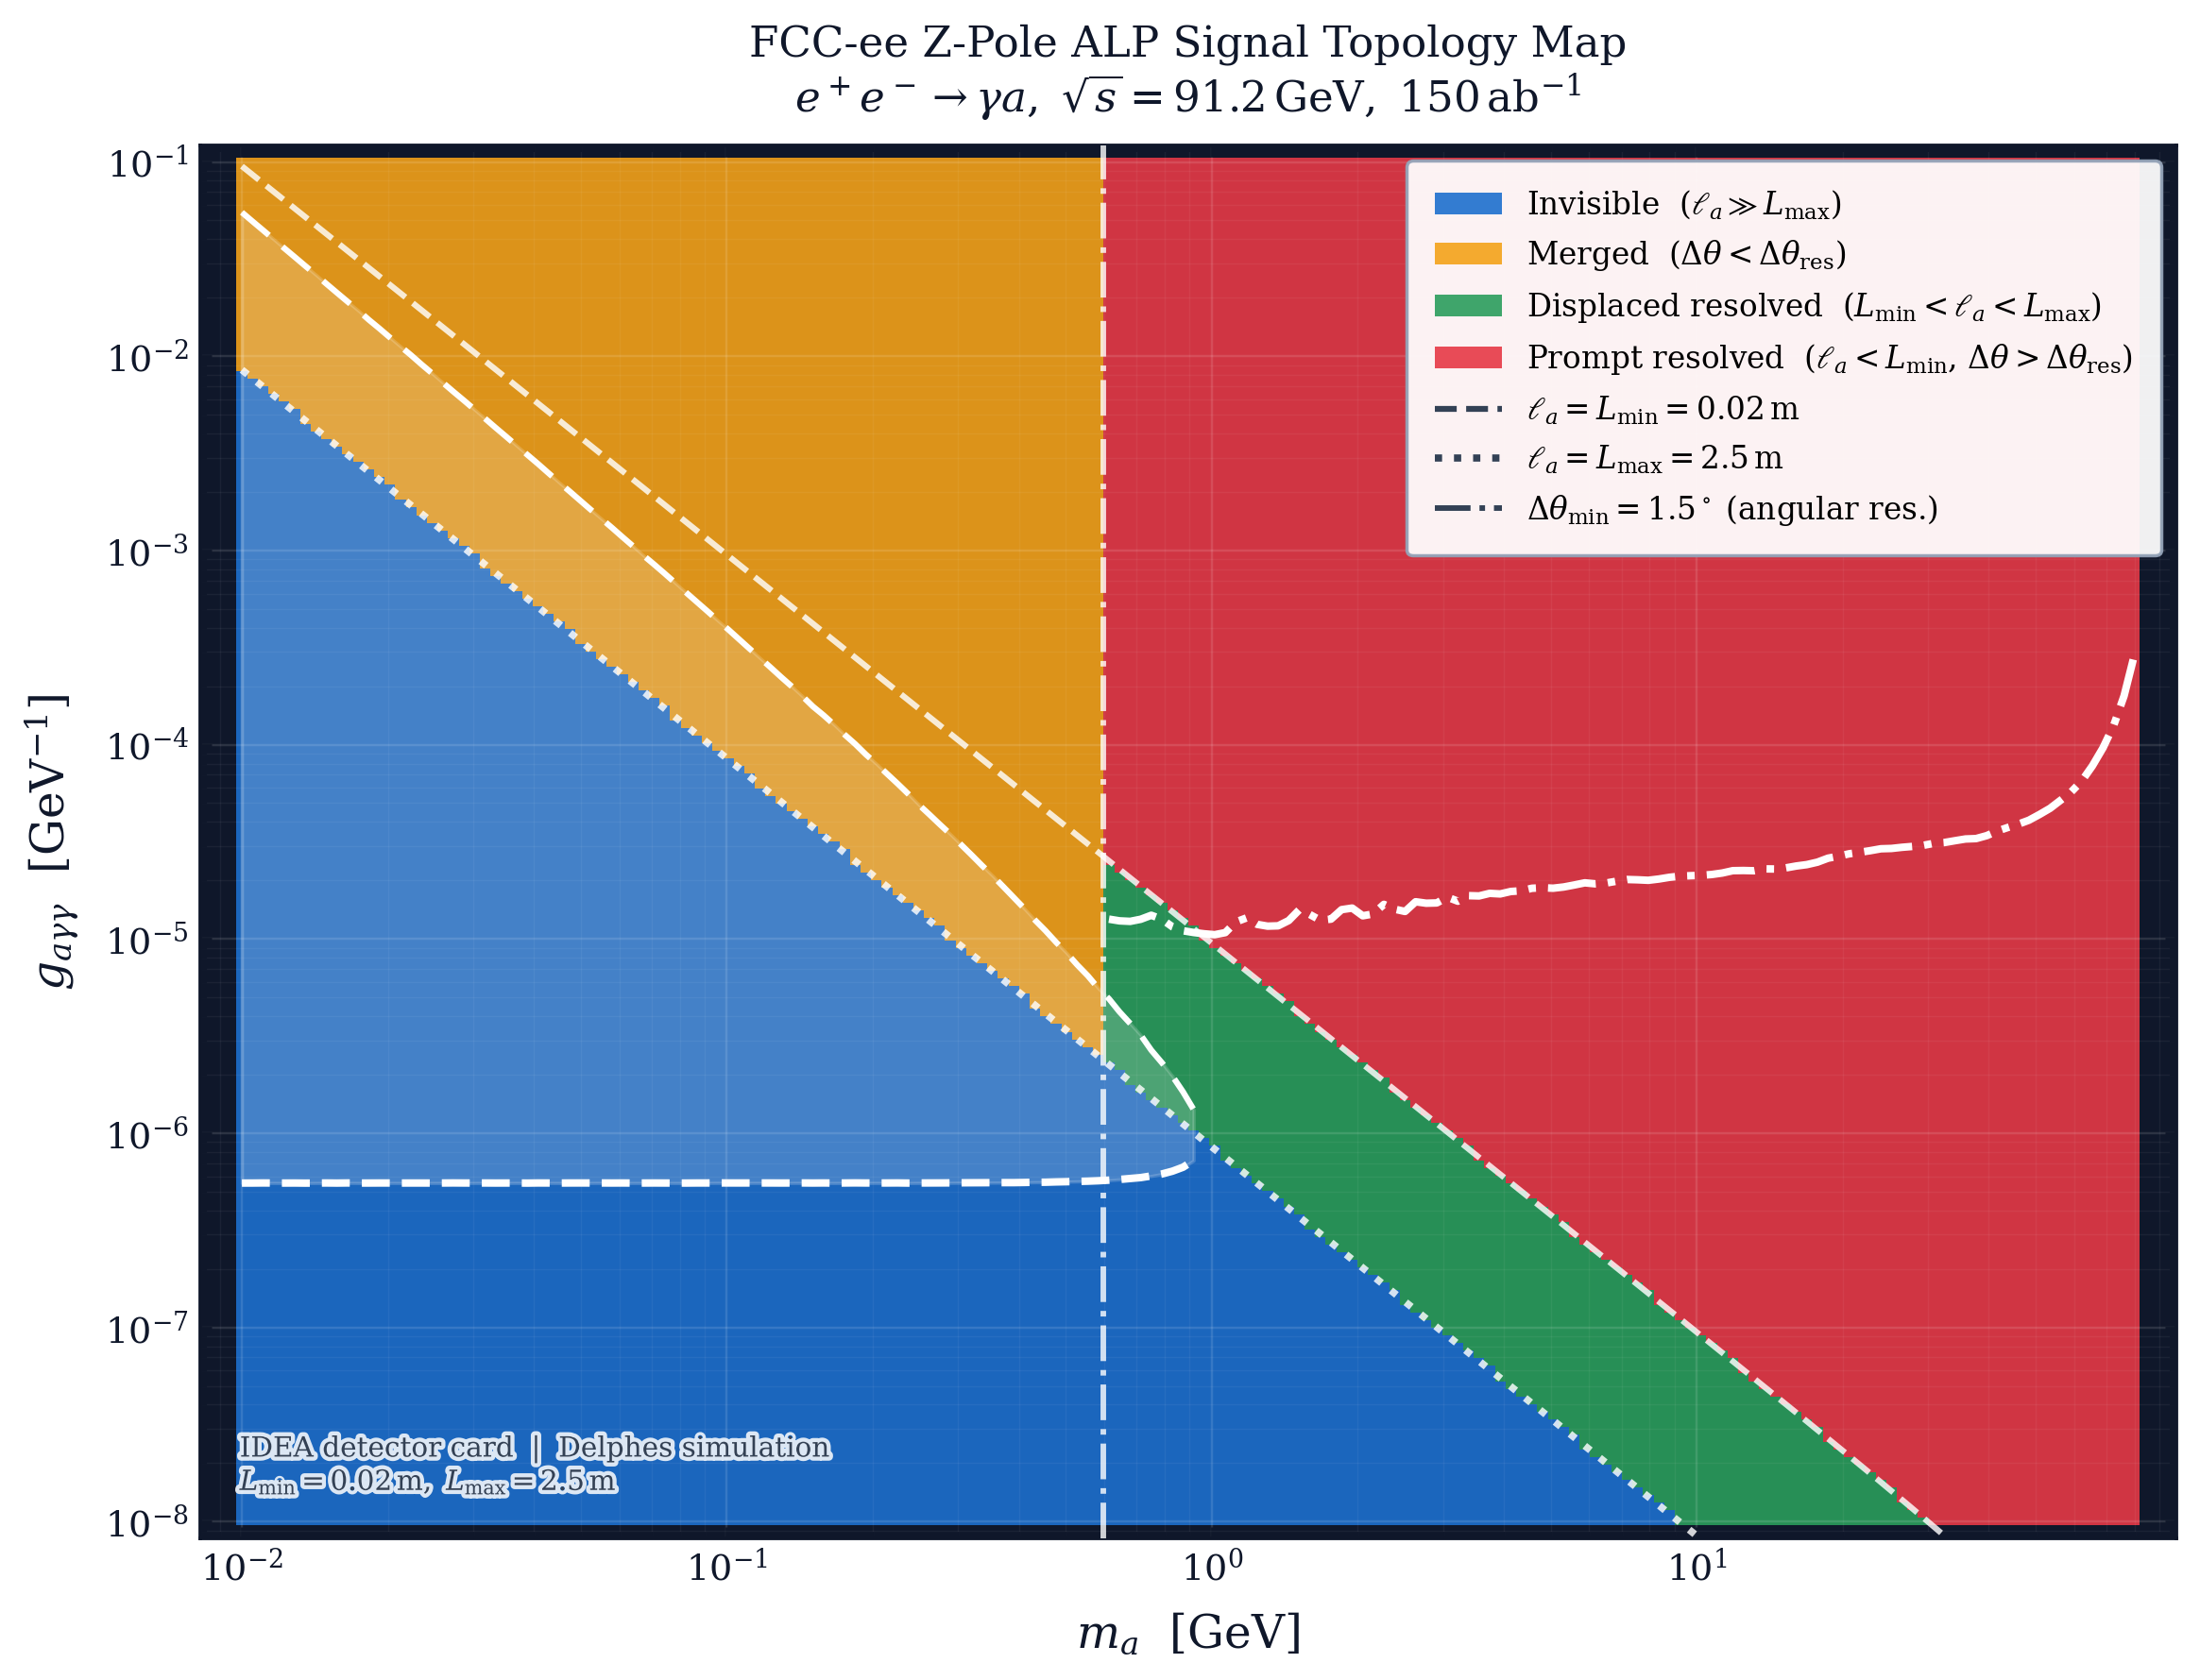
\includegraphics[width=0.75\textwidth]{figures/fccee_zpole_signature_classification.png}
    \caption{ALP signature classification in the $(m_{a}, g_{a\gamma\gamma})$ plane
    for the FCC-ee Z pole ($\sqrt{s} = 91.2\,\text{GeV}$) under IDEA detector assumptions.
    Dashed lines show the analytic $\ell_a = L_\mathrm{min}$ (prompt/displaced boundary)
    and $\ell_a = L_\mathrm{max}$ (displaced/invisible boundary) curves.
    The thin dash-dot curve shows the angular-resolution boundary
    $\Delta\theta = \Delta\theta_\mathrm{res} = 1.5^\circ$.
    Only the invisible and prompt-resolved signatures are used in the projected
    exclusion contours.}
    \label{fig:classification}
\end{figure}

Figure~\ref{fig:money} shows the main result: the projected FCC-ee Z-pole
exclusion contours overlaid on the current ALP-photon constraint landscape
from AxionLimits~\cite{AxionLimits}.

\begin{figure}[H]
    \centering
    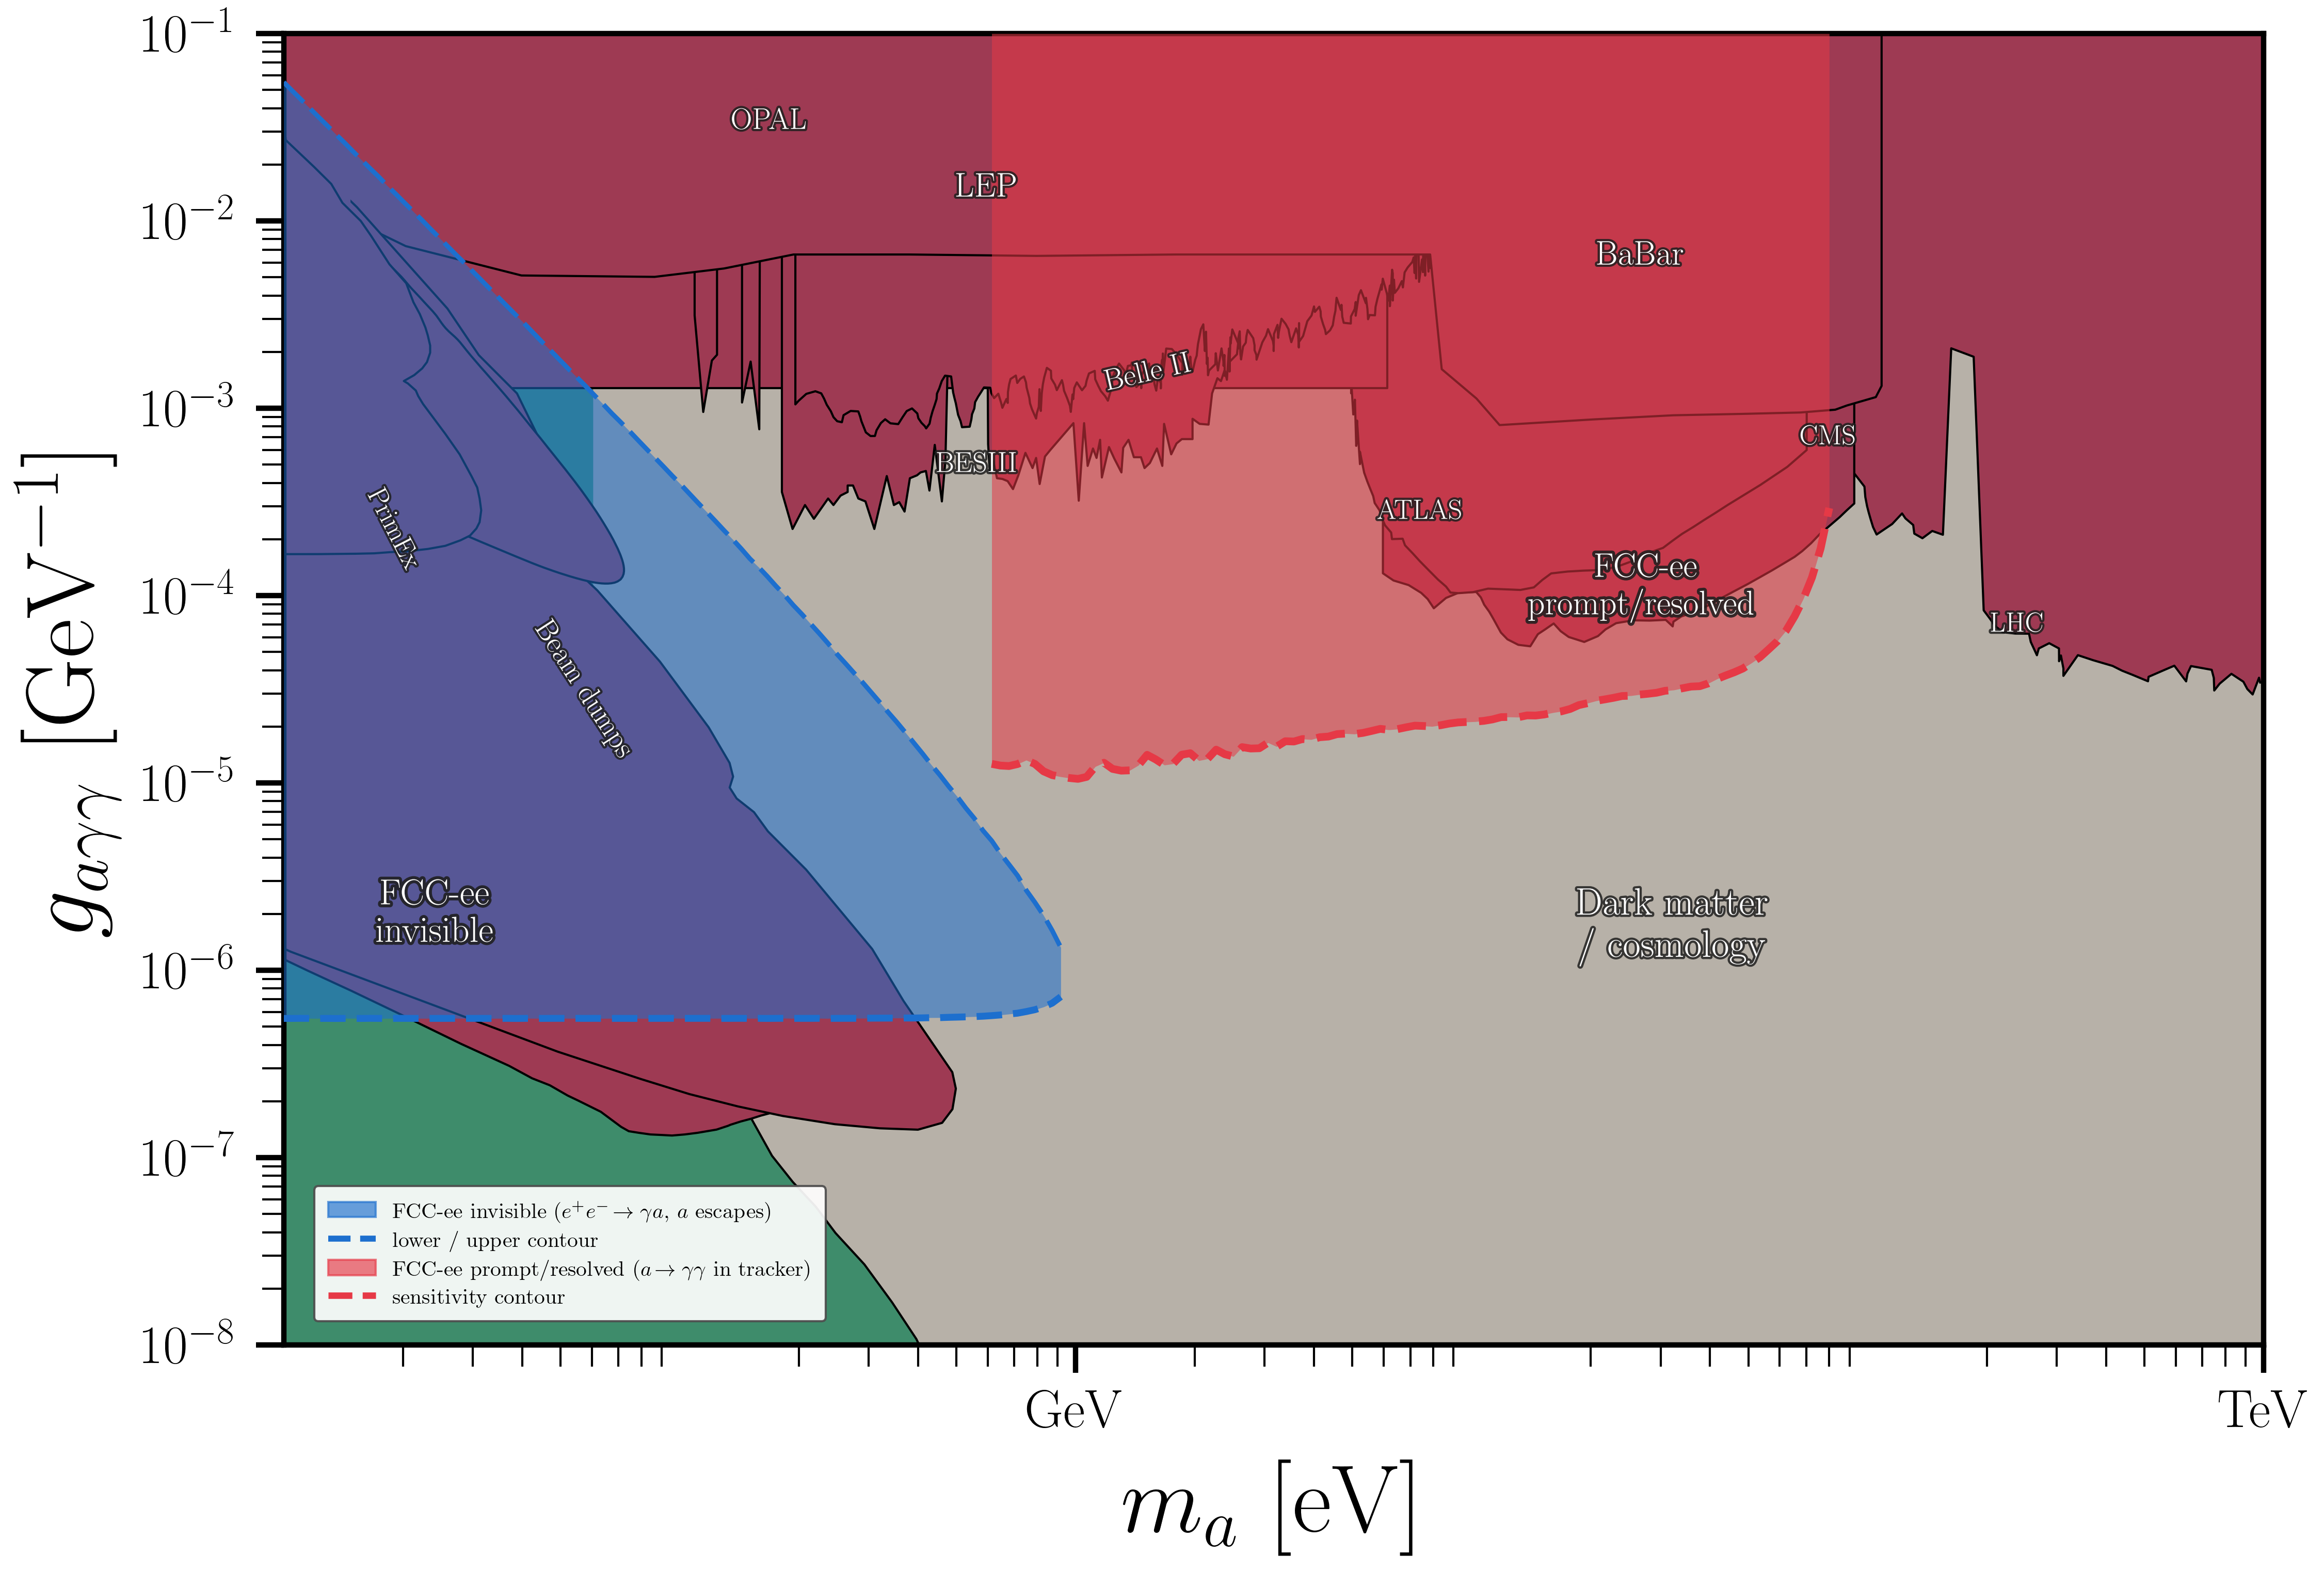
\includegraphics[width=\textwidth]{figures/money_plot_alp_full_closeup.png}
    \caption{Detector-relevant ALP-photon parameter space with FCC-ee Z-pole
    projected sensitivity. Existing constraints are shown as solid colored
    regions from AxionLimits~\cite{AxionLimits}. The translucent blue band is
    the FCC-ee invisible projection, bounded by the lower sensitivity contour
    and the upper short-lifetime contour. The translucent red region is the
    FCC-ee prompt-resolved projection, bounded by the dashed sensitivity
    contour.}
    \label{fig:money}
\end{figure}

The invisible channel reaches
$g_{a\gamma\gamma}\simeq5.5\times10^{-7}\,\text{GeV}^{-1}$ for
$m_{a}=0.01$--$0.92\,\text{GeV}$. It has a lower sensitivity branch and an
upper lifetime branch. The prompt-resolved channel starts at
$m_{a}\simeq0.61\,\text{GeV}$, set by the angular-resolution threshold, and
extends to $80\,\text{GeV}$. Its contour is roughly
$g_{a\gamma\gamma}\sim10^{-5}$--$3\times10^{-4}\,\text{GeV}^{-1}$ across the
mass range. In the $1$--$10\,\text{GeV}$ region this is about one to two orders
of magnitude below current Belle~II and BaBar bounds.

The external AxionLimits regions are used as context, not as one single
statistically identical exclusion. They include laboratory searches,
astrophysics, cosmology, dark matter assumptions, and QCD-axion model bands.
Our FCC-ee contour is a direct collider projection for the photophilic
benchmark only.

% ============================================================
\section{Discussion}
\label{sec:discussion}

The main strength of the result is that the same logic is checked at several
levels. The production cross section is analytic and verified with MadGraph.
The width and lifetime are fixed to the same convention in theory, Pythia, and
the parameter card. The Belle~II closure checks that the public contour can be
reconstructed. The FCC-ee signal points check that the final reconstructed
observables are where they should be: $M_{\gamma\gamma}\simeq m_{a}$ for
prompt-resolved events, and the recoil photon energy near
$(s-m_{a}^2)/(2\sqrt{s})$ for invisible events.

The result should still be read as a projection, not as an experimental limit.
The prompt-resolved branch and the lower invisible branch are the most robust,
because their detector corrections are close to one and their observables are
simple. The upper invisible branch is less precise because it is a lifetime
ceiling: the survival probability changes very quickly with
$g_{a\gamma\gamma}$, so small detector or ISR effects can move the contour.

The main missing pieces are also clear. We do not include machine backgrounds,
full detector systematics, reducible backgrounds from misidentified objects, or
higher-order corrections to the SM background rates. We also do not use the
merged and displaced signatures in the final limits. Those regions are real and
visible in the topology map, but they would need dedicated cluster-shape and
displaced-vertex studies. Finally, the present study cancels the tree-level
ALP--$Z$ coupling. Adding it would be a different two-coupling project, with
resonant $Z\to\gamma a$ production at the Z pole.

% ============================================================
\section{Conclusion}
\label{sec:conclusion}

We have computed projected 90\% CL exclusion contours for photophilic ALPs at
the FCC-ee Z pole, using analytic production and lifetime formulas corrected
with a MadGraph--Pythia--Delphes simulation pipeline. The invisible channel
reaches about $g_{a\gamma\gamma}=5.5\times10^{-7}\,\text{GeV}^{-1}$ for
$m_{a}=0.01$--$0.92\,\text{GeV}$. The prompt-resolved channel covers
$m_{a}=0.61$--$80\,\text{GeV}$ with sensitivity around
$10^{-5}$--$3\times10^{-4}\,\text{GeV}^{-1}$. The Belle~II public-contour
closure passes, and the FCC-ee pipeline includes detector-level signal checks
and SM background histograms. The main deliverable is therefore a complete and
clone-ready ALP simulation and projection pipeline, with a clear path to extend
the study to merged, displaced, and ALP--$Z$ signatures.

% ============================================================
\section*{Acknowledgements}

The author thanks the Nikhef computing cluster for providing the resources
used for the full-statistics Monte Carlo campaigns, and the AxionLimits
repository~\cite{AxionLimits} for the constraint landscape data.

% ============================================================
\bibliographystyle{unsrtnat}
\begin{thebibliography}{99}

\bibitem{Peccei1977}
R.~D.~Peccei and H.~R.~Quinn,
\textit{CP conservation in the presence of pseudoparticles},
Phys.\ Rev.\ Lett.\ \textbf{38}, 1440 (1977).

\bibitem{Weinberg1978}
S.~Weinberg,
\textit{A new light boson?},
Phys.\ Rev.\ Lett.\ \textbf{40}, 223 (1978).

\bibitem{Wilczek1978}
F.~Wilczek,
\textit{Problem of strong P and T invariance in the presence of instantons},
Phys.\ Rev.\ Lett.\ \textbf{40}, 279 (1978).

\bibitem{Jaeckel2010}
J.~Jaeckel and A.~Ringwald,
\textit{The low-energy frontier of particle physics},
Annu.\ Rev.\ Nucl.\ Part.\ Sci.\ \textbf{60}, 405 (2010),
[\href{https://arxiv.org/abs/1002.0329}{arXiv:1002.0329}].

\bibitem{Brivio2017}
I.~Brivio \textit{et al.},
\textit{ALPs effective field theory and collider signatures},
Eur.\ Phys.\ J.\ C \textbf{77}, 572 (2017),
[\href{https://arxiv.org/abs/1701.05379}{arXiv:1701.05379}].

\bibitem{Dolan2017}
M.~J.~Dolan, T.~Erber, F.~Kahlhoefer, and M.~Schmidt-Hoberg,
\textit{Searching for ALPs with LEP, the LHC and a future circular collider},
JHEP \textbf{10}, 079 (2017),
[\href{https://arxiv.org/abs/1709.03453}{arXiv:1709.03453}].

\bibitem{Jaeckel2016}
J.~Jaeckel and M.~Thormaehlen,
\textit{Distinguishing axion models with the axion-photon coupling},
Phys.\ Rev.\ D \textbf{95}, 015010 (2017),
[\href{https://arxiv.org/abs/1612.00034}{arXiv:1612.00034}].

\bibitem{FCCee_CDR}
A.~Abada \textit{et al.}\ (FCC Collaboration),
\textit{FCC-ee: The lepton collider},
Eur.\ Phys.\ J.\ Special Topics \textbf{228}, 261 (2019),
[\href{https://arxiv.org/abs/1905.05078}{arXiv:1905.05078}].

\bibitem{FCC_Physics}
A.~Abada \textit{et al.}\ (FCC Collaboration),
\textit{FCC physics opportunities},
Eur.\ Phys.\ J.\ C \textbf{79}, 474 (2019),
[\href{https://arxiv.org/abs/1905.05078}{arXiv:1905.05078}].

\bibitem{IDEA}
A.~Abada \textit{et al.},
\textit{IDEA: A detector concept for FCC-ee},
Eur.\ Phys.\ J.\ Special Topics \textbf{228}, 1107 (2019).

\bibitem{Belle2}
I.~Adachi \textit{et al.}\ (Belle~II Collaboration),
\textit{Search for axion-like particles produced in $e^+e^-$ collisions at Belle II},
Phys.\ Rev.\ Lett.\ \textbf{130}, 231801 (2023),
[\href{https://arxiv.org/abs/2206.07598}{arXiv:2206.07598}].

\bibitem{AxionLimits}
C.~O'Hare,
\textit{cajohare/AxionLimits: AxionLimits},
Zenodo (2020),
\href{https://doi.org/10.5281/zenodo.3932430}{DOI: 10.5281/zenodo.3932430},
\url{https://cajohare.github.io/AxionLimits/}.

\bibitem{MG5}
J.~Alwall \textit{et al.},
\textit{The automated computation of tree-level and next-to-leading order differential
cross sections, and their matching to parton showers},
JHEP \textbf{07}, 079 (2014),
[\href{https://arxiv.org/abs/1405.0301}{arXiv:1405.0301}].

\bibitem{Pythia8}
T.~Sjöstrand \textit{et al.},
\textit{Introduction to \textsc{Pythia}~8.2},
Comput.\ Phys.\ Commun.\ \textbf{191}, 159 (2015),
[\href{https://arxiv.org/abs/1410.3012}{arXiv:1410.3012}].

\bibitem{Delphes}
J.~de~Favereau \textit{et al.}\ (DELPHES~3 Collaboration),
\textit{DELPHES 3: A modular framework for fast simulation of a generic detector},
JHEP \textbf{02}, 057 (2014),
[\href{https://arxiv.org/abs/1307.6346}{arXiv:1307.6346}].

\bibitem{Cowan2011}
G.~Cowan, K.~Cranmer, E.~Gross, and O.~Vitells,
\textit{Asymptotic formulas for likelihood-based tests of new physics},
Eur.\ Phys.\ J.\ C \textbf{71}, 1554 (2011),
[\href{https://arxiv.org/abs/1007.1727}{arXiv:1007.1727}].

\end{thebibliography}

% ============================================================
\appendix
\section*{Appendix: Contribution Statement}

Iñaki Pardo led the physics study, repository organization, simulation
campaigns, analysis development, validation, plotting, and writing. The project
was developed in collaboration with project partners and with Codex-assisted
implementation and documentation work. External software, models, detector
cards, constraint data, and papers are credited in the repository provenance
report and bibliography.

\end{document}
